% Header
\renewcommand\evenpagerightmark{{\scshape\small Chapter 6}}
\renewcommand\oddpageleftmark{{\scshape\small Improved RPC investigation and preliminary electronics studies}}

\renewcommand{\bibname}{References}

\hyphenation{}

\chapter[Improved RPC investigation and preliminary electronics studies]%
{Improved RPC investigation and preliminary electronics studies}
\label{chapt6}

	The extension in the endcap of the RPC sub-system towards higher pseudo-rapidity will bring the new detectors to be exposed to much more intense background radiations due to the proximity of the detectors with the beam line (Figure~\ref{fig:Dose}). The challenge will be to produce high counting rate detectors with limited ageing rate to ensure a stable operation of the detector over a period longer than ten years. In Chapter~\ref{chapt4} was discussed the influence of the detector design (number and thickness of gas volumes, OR system, etc...) on the charge deposition and rate capability. Nevertheless, this question can also be addressed from the electronics point of view as a better signal-to-noise ratio would also mean the possibility to greatly lower the charge threshold on the signals to be detected, allowing to use the detector at lower gain, hence lowering the charge deposition per avalanche in the gas volume. Cardarelli showed that the production of low-noise fast FEEs could help decreasing the charge deposition per avalanche at working voltage by an order of magnitude, virtually increasing the life expectancy of such a detector in the same way~\cite{CARDARELLI2012}.

\section{FEE candidates for the production of iRPCs}
\label{chapt6:sec:candidates}

	The extension of the third of fourth endcap disks with \acl{iRPC}s has been presentated in Chapter~\ref{chapt:3} together with the expected background levels (Figure~\ref{fig:iRPC-Rate}). An important piece of these iRPCs will be the \acl{FEE} that will equip the chambers. A fast, low-jitter and low-charge sensitive electronics will help reducing further the charge deposition in the detector by making it possible to operate at lower gain.
	
	In the context of the CMS Muon Upgrade, two FEE solutions have been considered to equip the iRPCs. The baseline for the RPC upgrade is based on the PETIROC ASIC, initially for \acf{ToF} applications. A back-up solution is also under study and focusses on a new low-noise preamplifier designed in INFN laboratories in Rome to replace the preamplification stage of the already existing CMS RPC \acl{FEB}.

	The FEEs that are foreseen to equip the new RPCs need to be able to detect charges as small as \SI{10}{fC}. Not only the new electronics need to be fast and reliable, they also should be able to sustain the high radiation the detectors will be subjected to in the region closest to the beam.
	
	\subsection{CMS RPCROC: the RPC upgrade baseline}
	\label{chapt6:ssec:RPCROC}
	
	Designed by Weeroc, a spin-off company from the french OMEGA laboratory, the PETIROC 2A consits in a fast and low jitter 32-channel ASIC originally developed to read-out \acf{SiPM} in ToF applications and that allows for precise time measurements~\cite{PETIROCIEEE,PETIROCTWEPP}. The ASIC uses an AMS \SI{350}{ns} SiGe technology. The block diagram of the ASIC is showed on Figure~\ref{fig:PETIROCASIC}. A 10-bit DAC allows to adjust the trigger level in a dynamical range spanning from 0.5 to a few tens of photoelectrons and a 6-bit DAC to adjust the response of each individual channel to similar a level.
	
	\begin{figure}[H]
		\centering
		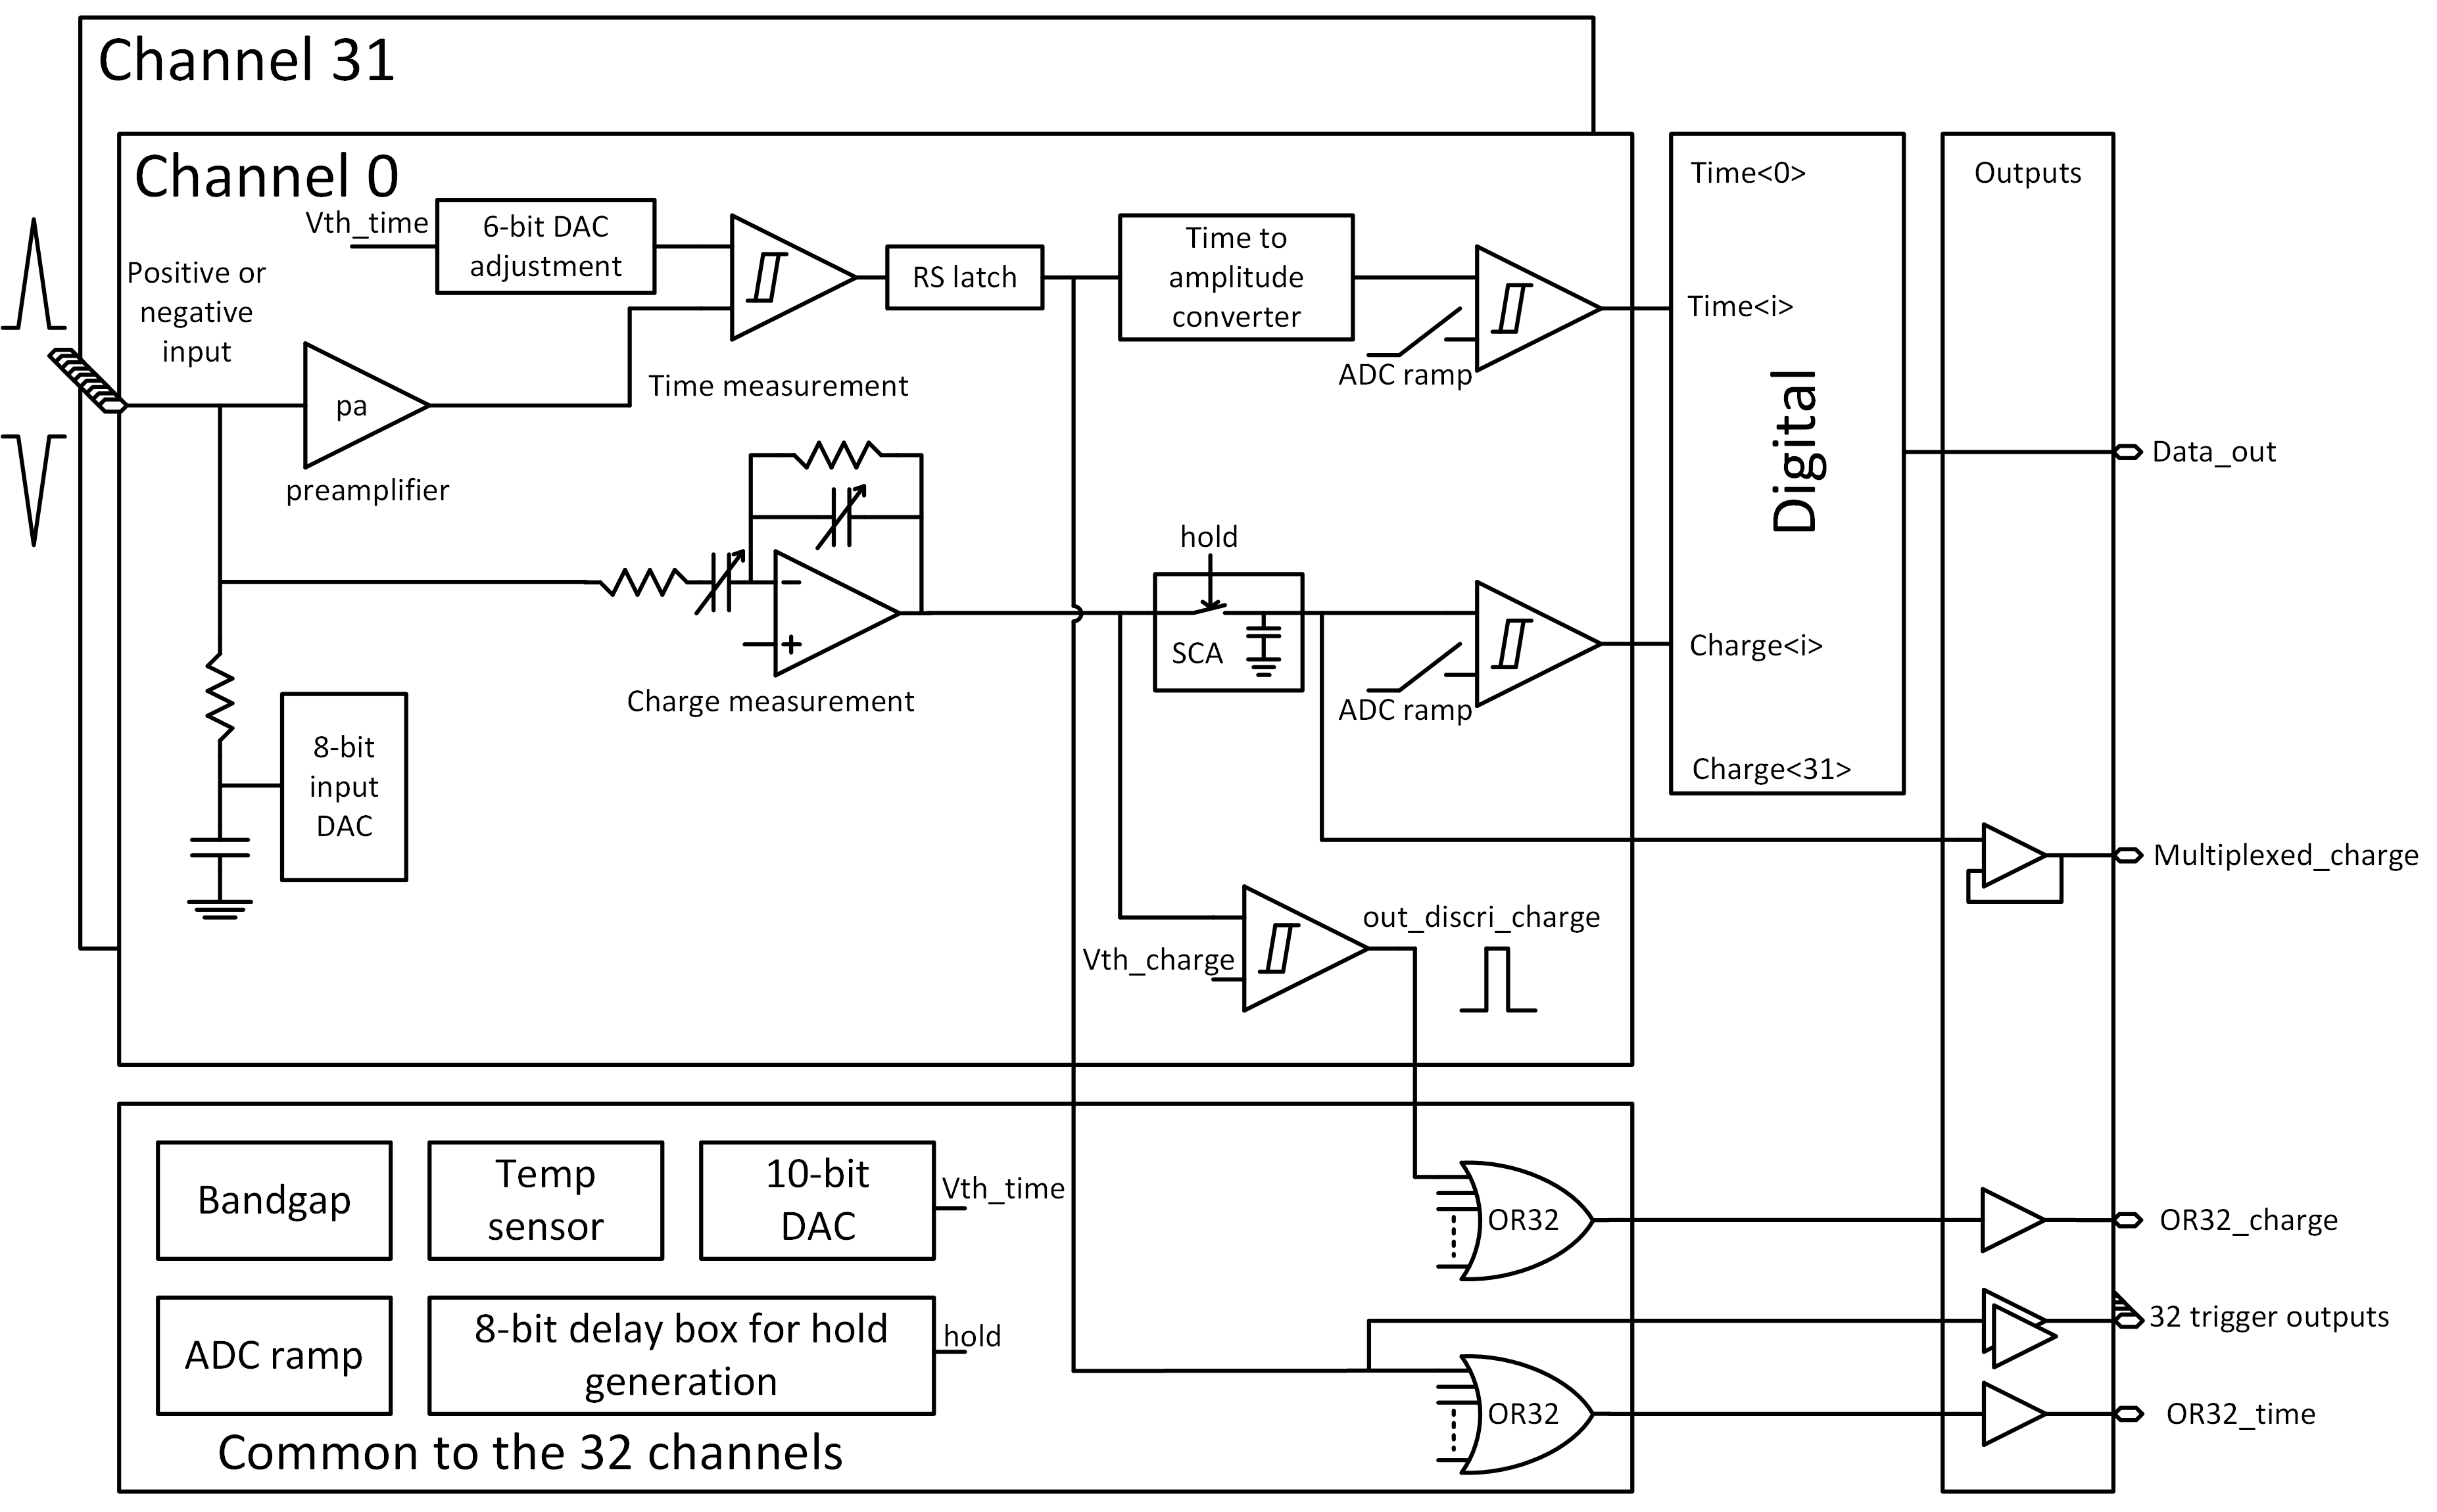
\includegraphics[width = \linewidth]{fig/chapt6/petiroc2.png}\\
		\caption{\label{fig:PETIROCASIC} PETIROC 2A block diagram.}
	\end{figure}
	
	Nevertheless, in order to adapt this ASIC to CMS, modifications were brought to the PETIROC~\cite{PHASEIITP}. In the new CMS RPCROC, the measurement of the charge will be performed by a TimeOverTechnic, taking profit of the capacity the ASIC has in measuring both the leading and trailing edges of the input signals. The dynamic range will be expanded towards lower values to allow for the detection of charges as low as \SI{10}{fC}. Due to the radiation levels that are foreseen at the level of the iRPCs, the SiGe technology will be replaced by the Taiwan Semiconductor Manufacturing Company (TSMC) \SI{130}{nm} CMOS, to increase its radiation hardness while keeping fast pre-amplification and discrimination with a very low jitter that can reach less than \SI{20}{ps} if no internal clock is used, as can be seen from Figure~\ref{fig:jitter}. The ASIC is associated with an FPGA which purpose is to measure time thanks to a TDC with a time resolution of 50-100 \si{ps} developed by Tsinghua University and that will provide a measurement of the signal position along the strip with a precision of a few \si{cm} by measuring the signal timing on both ends of the strips. In order to read-out all 96 strips, 3 ASICs and 3 TDCs, each having an increased number of 64-channels, are hosted on a FEB attached to the chamber.

	\begin{figure}[H]
		\centering
		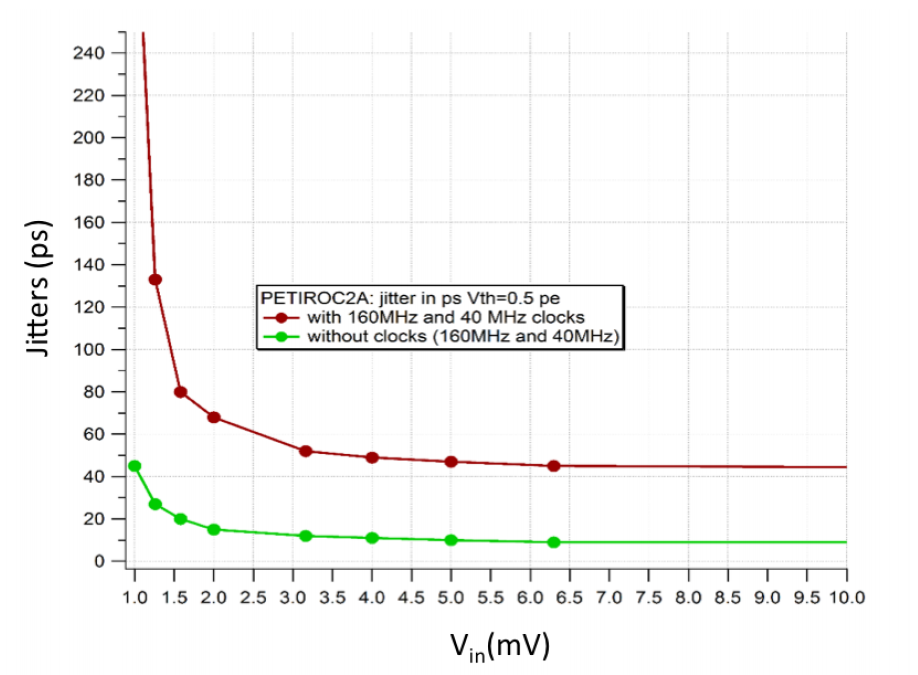
\includegraphics[width=0.8\plotwidth]{fig/chapt6/jitter-PETIROC.png}
		\caption{\label{fig:jitter} The PETIROC time jitter as a function of the input signal amplitude, measured with and without internal clocks.}
	\end{figure}

	\subsection{INFN \acl{FEE}: a robust back-up solution}
	\label{chapt6:ssec:INFN}

\section{Preliminary tests at CERN}
\label{chapt6:sec:Preliminary}

	\subsection{INFN preamplifiers}
	\label{chapt6:ssec:INFN-Prelim}
	
	INFN electronics were the first ones to be tested by CMS RPC group in collaboration with colleagues from INFN Roma working in the ATLAS RPC group. Indeed, at first the electronics only consisted in a new low-noise preamplifier produced by the team of Cardarelli with the purpose of equipping the new generation of ATLAS RPCs~\cite{CARDARELLI2013}. The tests with CMS RPCs were performed in February 2013 outside of the old GIF facility presented in Chapter~\ref{chapt5:ssec:GIF}. Four preamplifier channels were lended by Cardarelli to equip four CMS RPC channels as presented in Figure~\ref{fig:INFN-preamp}. They were directly connected to the strips for the signals induced by muons passing through the gas volume of the chamber to be amplified. The output was then sent to a discriminator to digitize the signals and filter out the noise by tuning the threshold level.
	
	\begin{figure}[H]
		\centering
		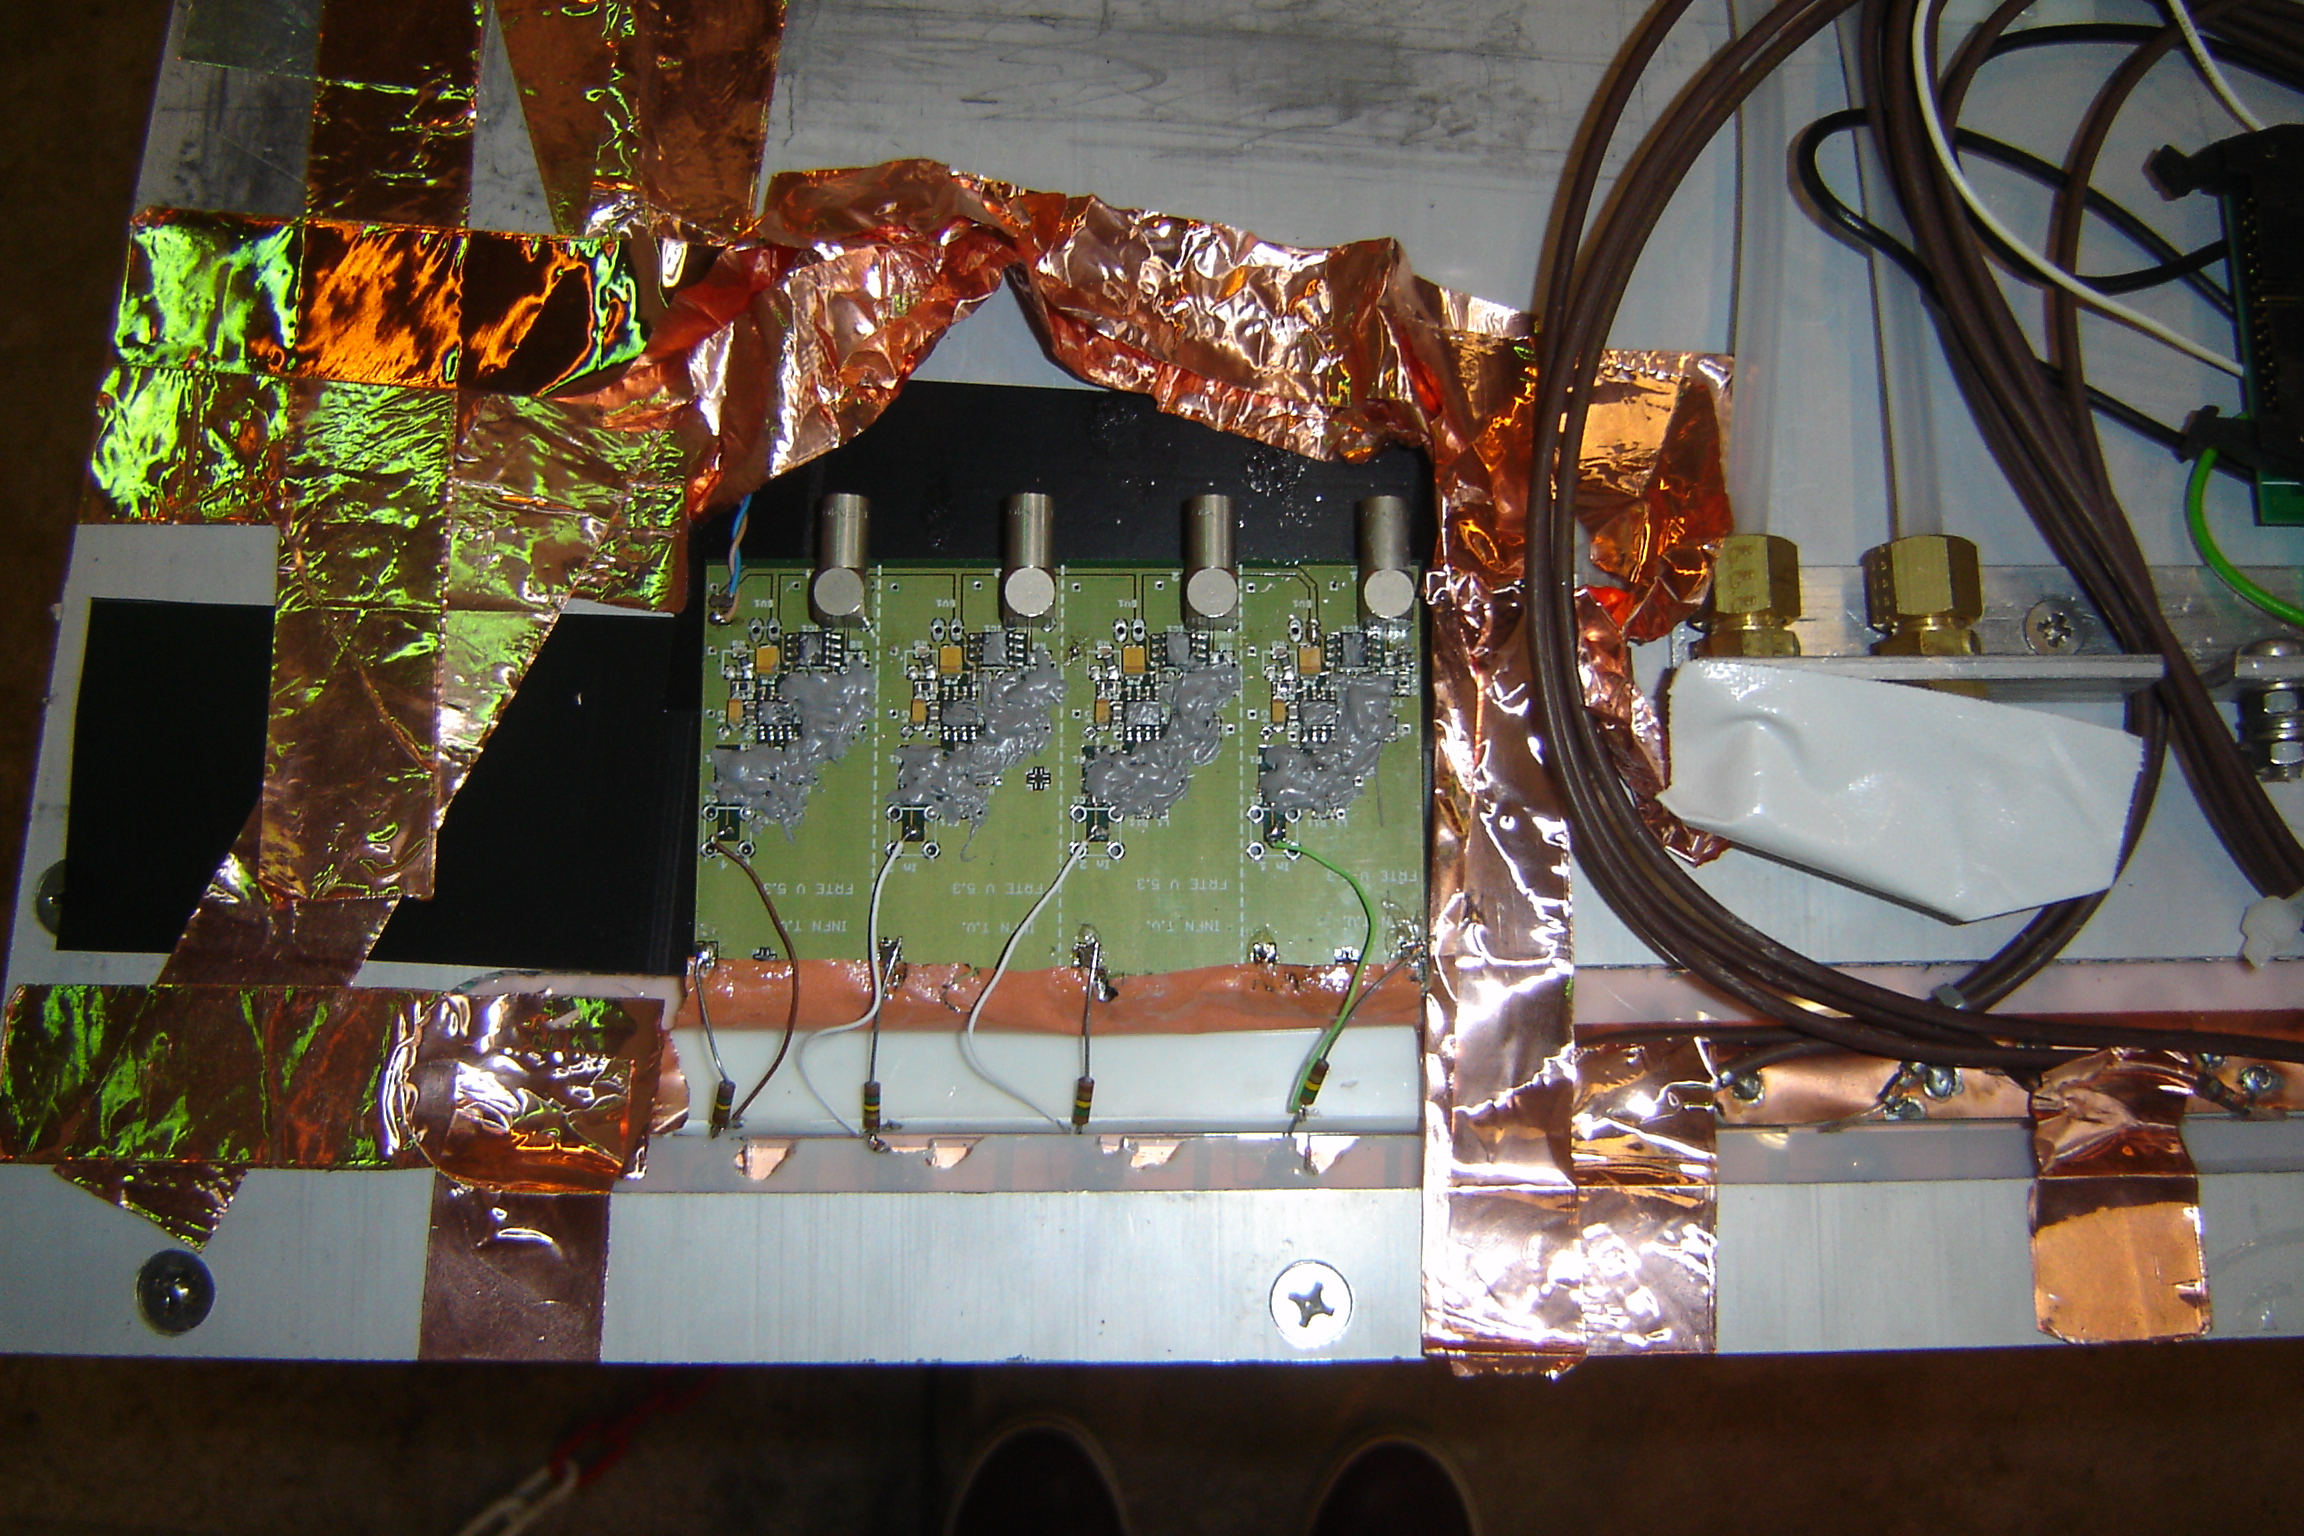
\includegraphics[width=0.8\plotwidth]{fig/chapt6/INFN-Preamp-2013.JPG}
		\caption{\label{fig:INFN-preamp} The four channels of INFN preamplifiers are mounted directly on a CMS RPC and connected to the four outermost read-out strips of the detector.}
	\end{figure}
	
	The performance of the chamber equipped with these new preamplifiers was compared to the performance of CMS FEEs. The experimental setup used is described in Figure~\ref{Setup-GIF}. PMTs a little less wide than four strips were used to trigger the data tacking. Two pairs were used in coïncidence on both the strips connected to the INFN preamplifiers and to the ones connected to the CMS FEEs. An extra PMT, placed perpendicularly to the rest of the setup at the bottom of the setup was used to detect potential showers and send VETO signals if necessary. A last PMT was used close to the power supplies to measure and discard signals due to electromagnetic noise and is not visible on the pictures. Finally, after discrimination, the output of the INFN preamplifiers together with the signals from the CMS FEEs were sent to scalers to count the detected signals versus the number of trigger coïncidences as no DAQ software was available at the time. The full pulse processing for this experiment is shown in Figure~\ref{fig:Pulse-Processing}.
	 
	\begin{figure}[H]
		\begin{subfigure}{\linewidth}
		    \centering
			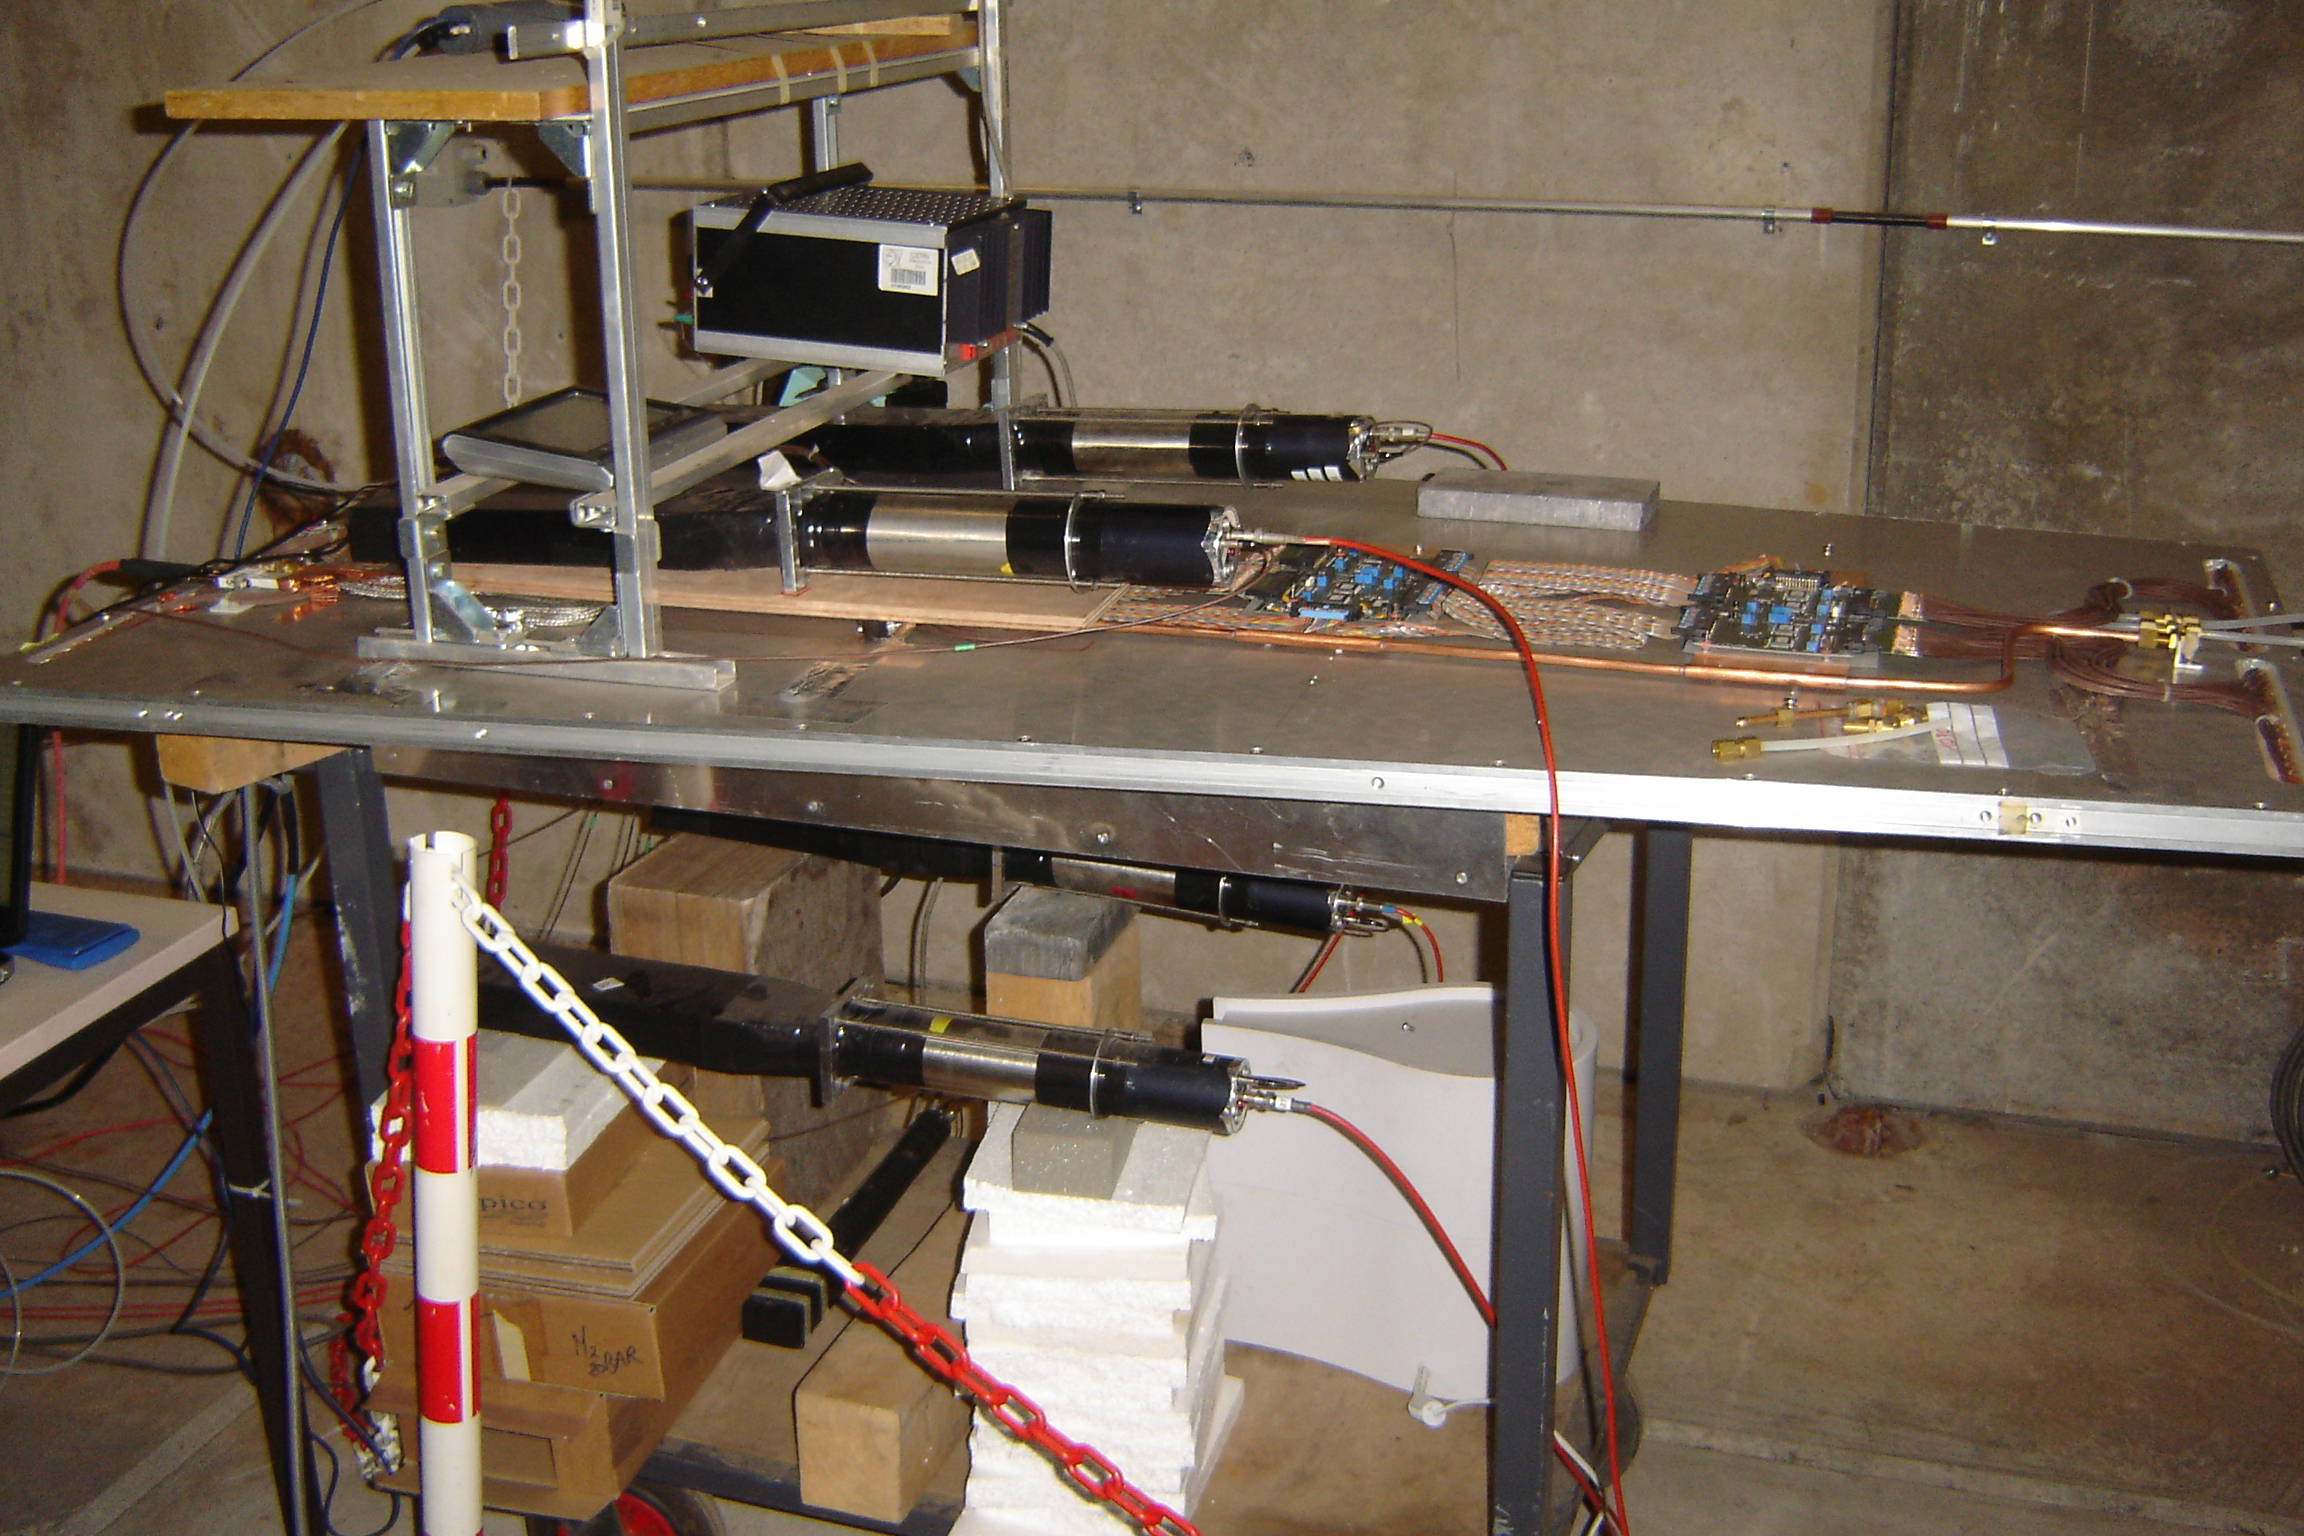
\includegraphics[width = 0.7\linewidth]{fig/chapt6/Setup-GIF-side.JPG}
			\caption{\label{fig:Setup-GIF:A}}
		\end{subfigure}
		\begin{subfigure}{0.5\linewidth}
		    \centering
			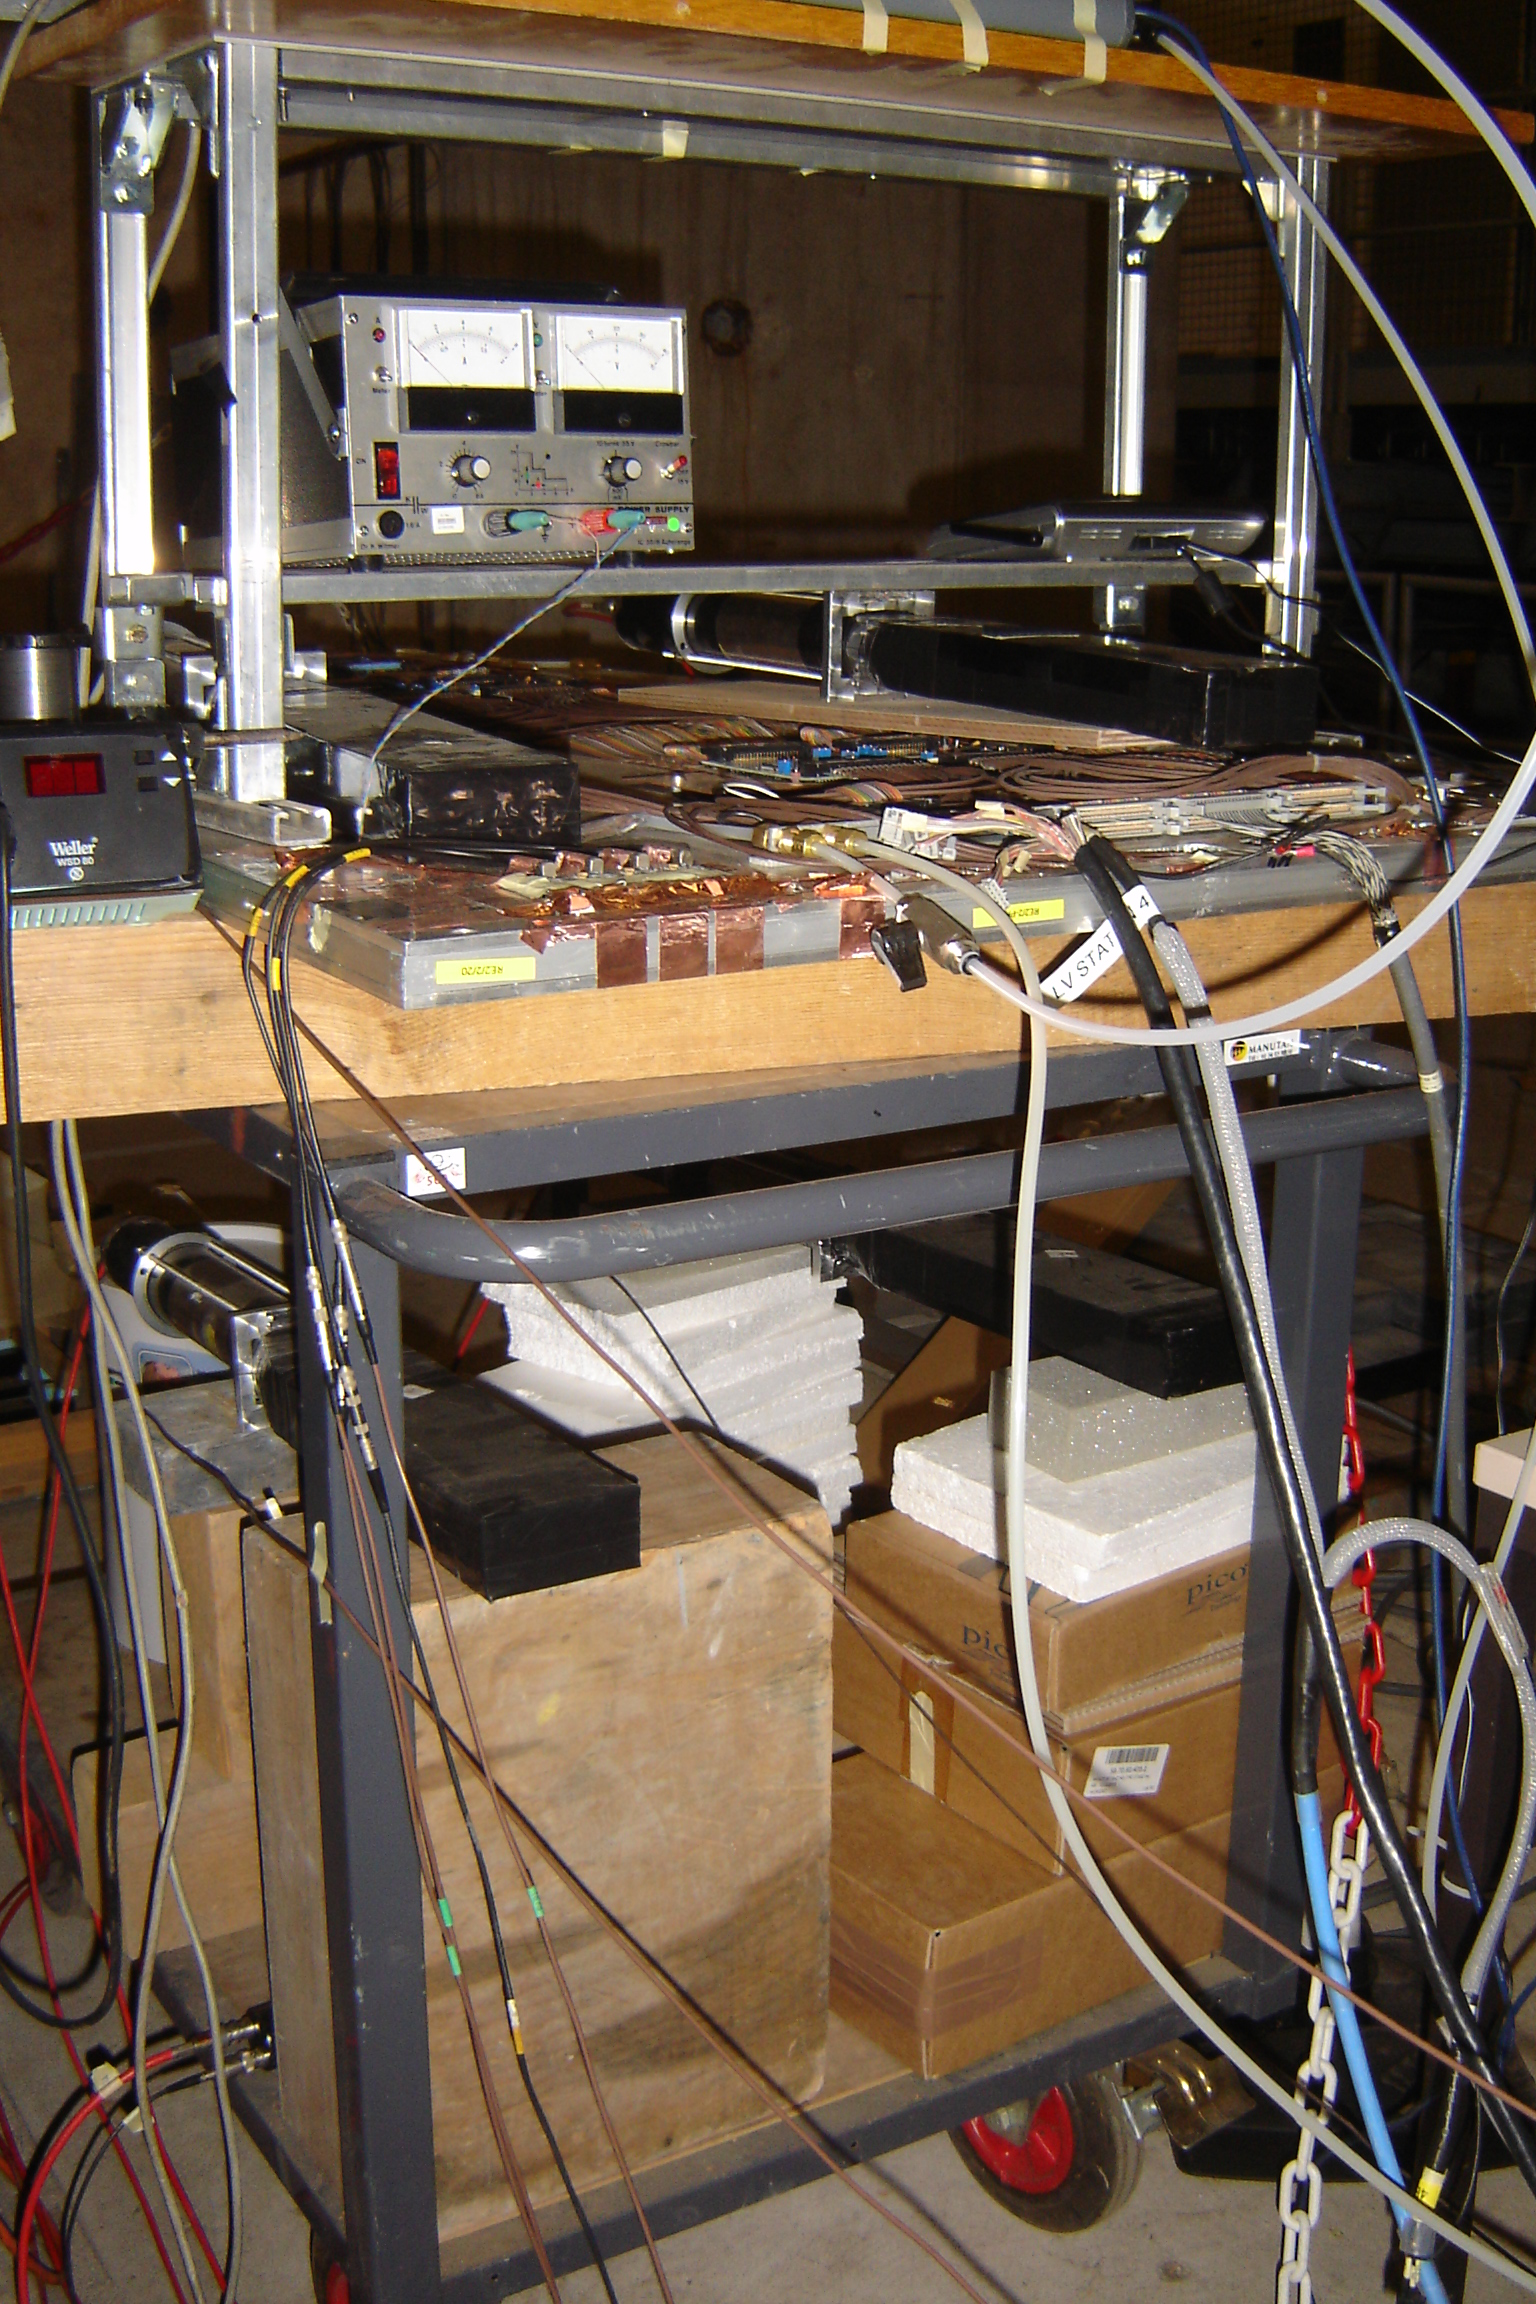
\includegraphics[width = 0.8\linewidth]{fig/chapt6/Setup-GIF-front.JPG}
			\caption{\label{fig:Setup-GIF:B}}
		\end{subfigure}
		\begin{subfigure}{0.5\linewidth}
		    \centering
			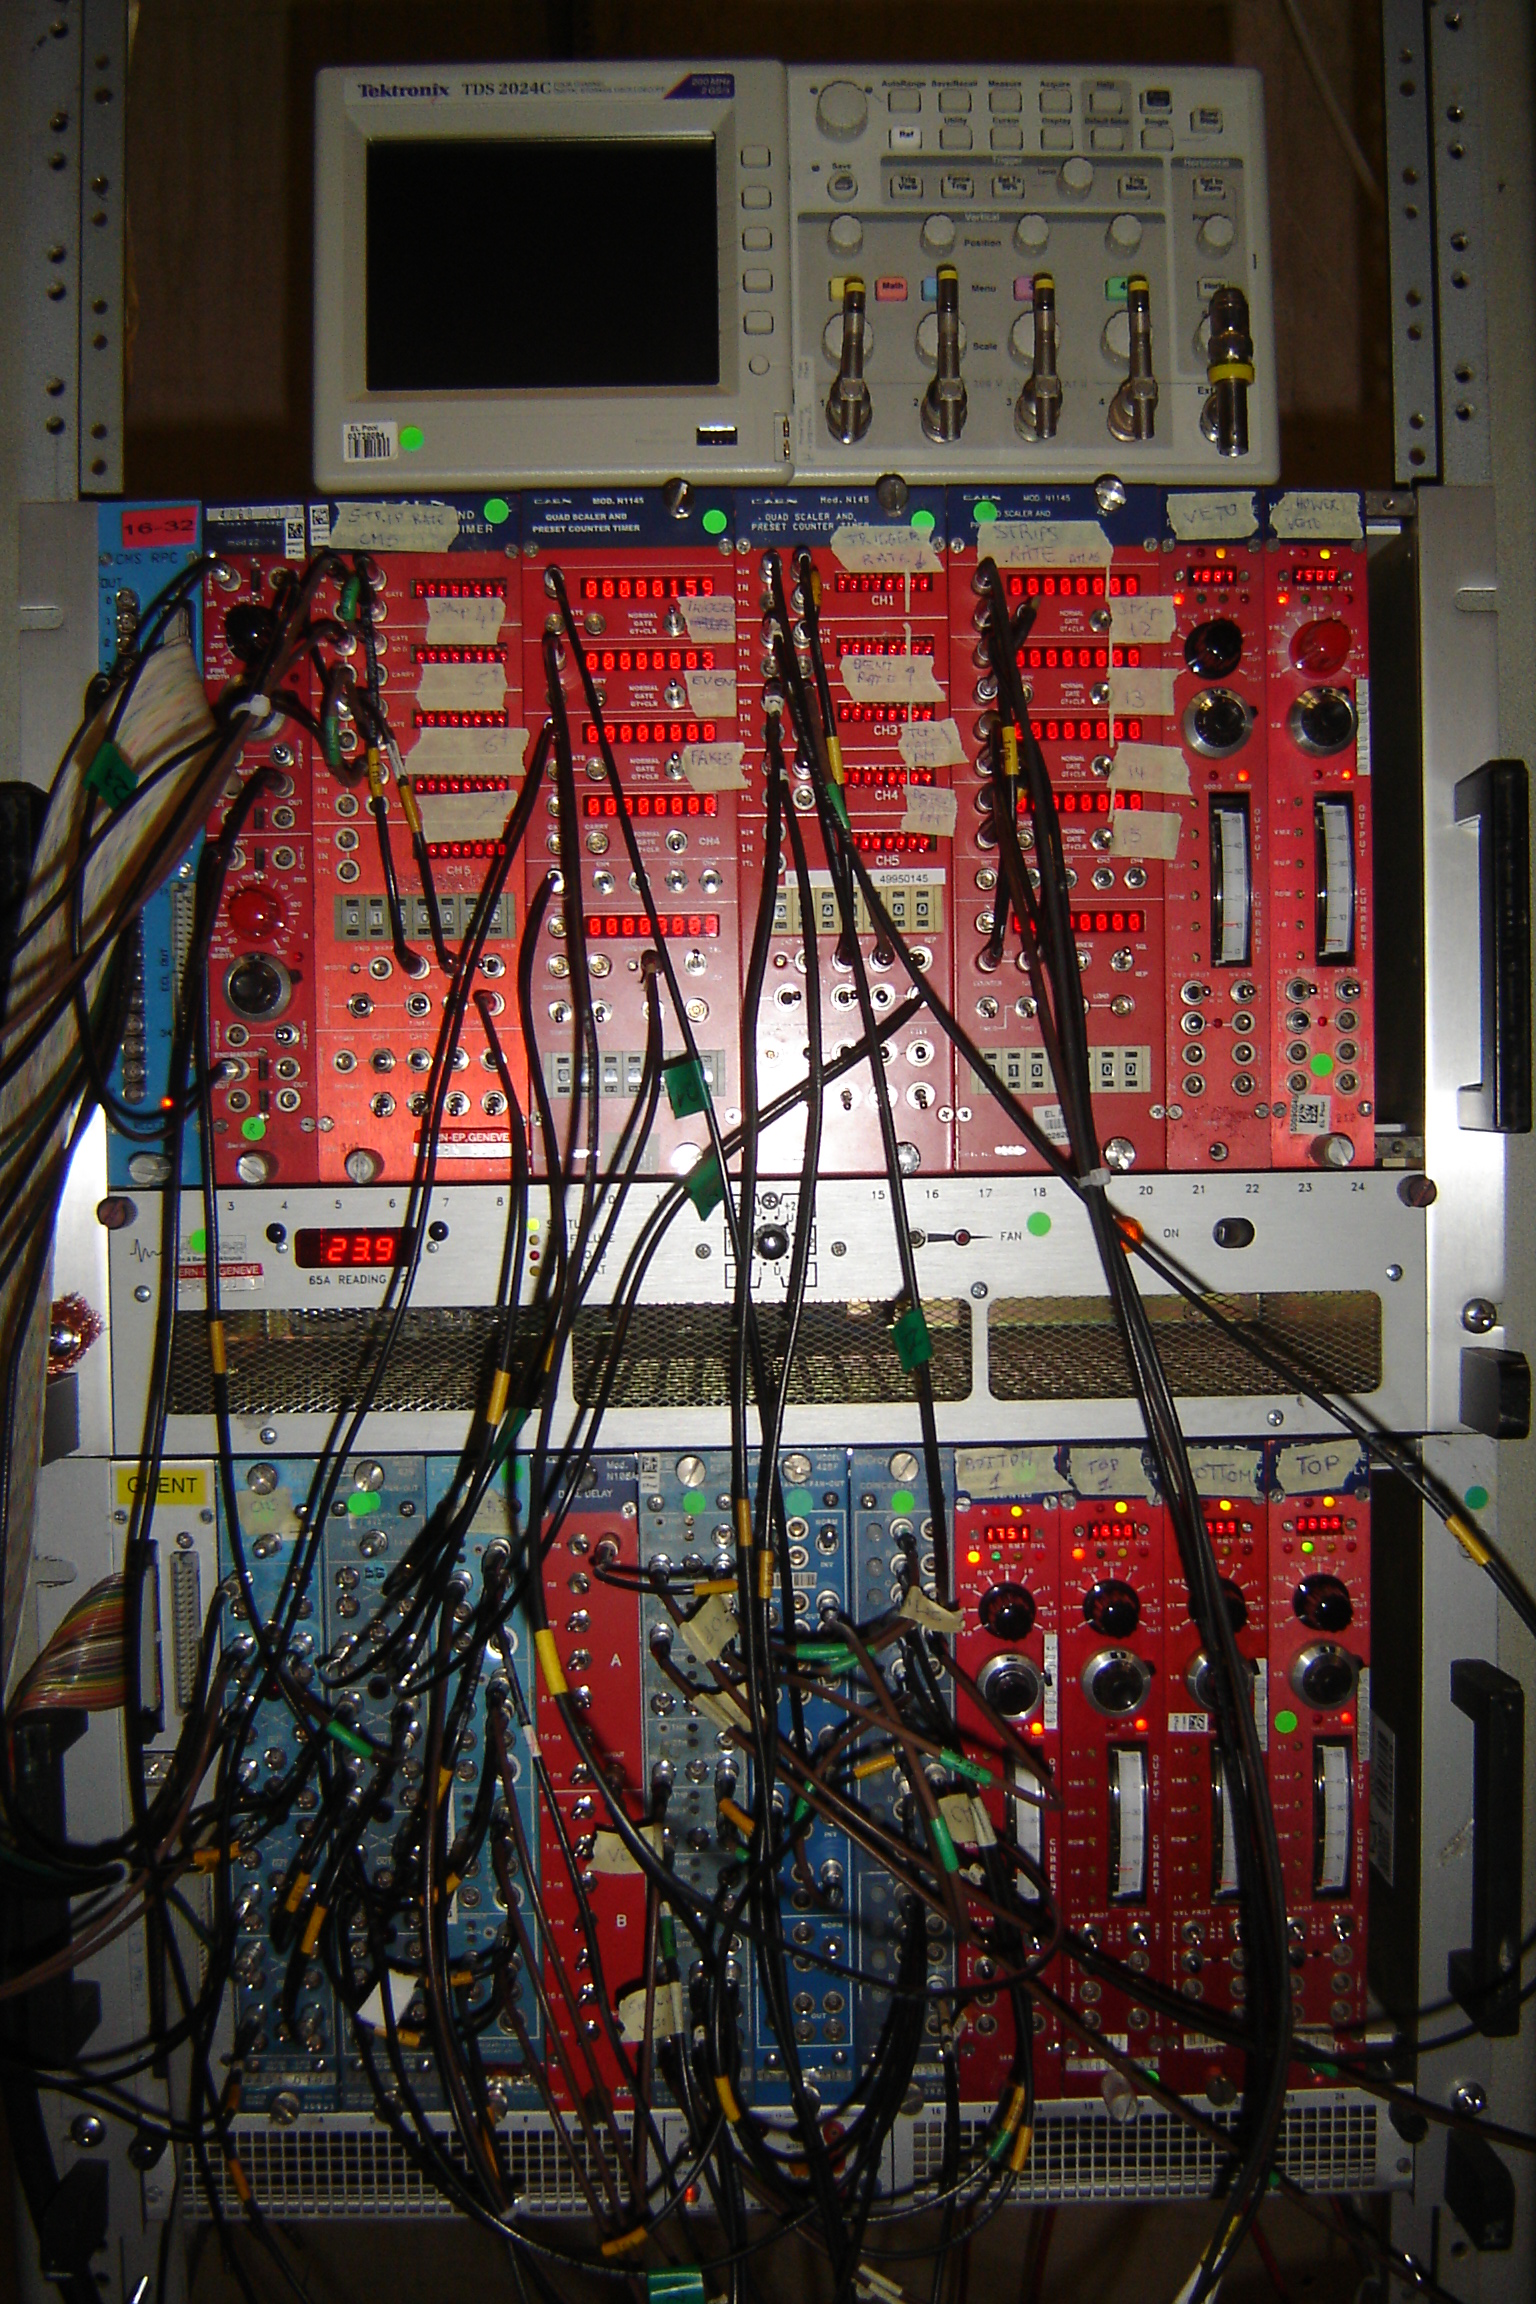
\includegraphics[width = 0.8\linewidth]{fig/chapt6/Pulse-processing-GIF.JPG}
			\caption{\label{fig:Setup-GIF:C}}
		\end{subfigure}
		\caption{\label{fig:Setup-GIF} Experimental setup used to test the INFN preamplifier with respect to the CMS FEEs.}
    \end{figure}
	 
	\begin{figure}[H]
		\begin{subfigure}{.5\linewidth}
		    \centering
			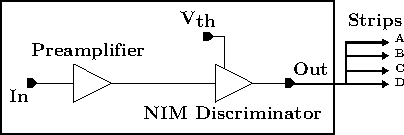
\includegraphics[width = 0.9\linewidth]{fig/chapt6/atlas-block-diagram-2013.pdf}
			\caption{\label{fig:Pulse-Processing:A}}
		\end{subfigure}
		\begin{subfigure}{.5\linewidth}
		    \centering
			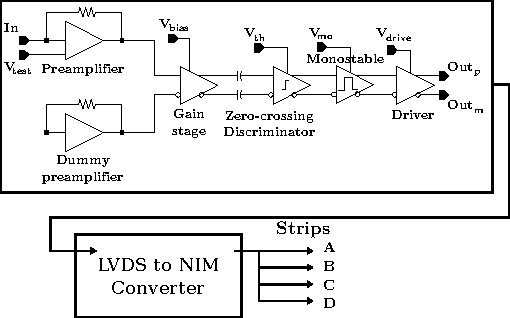
\includegraphics[width = 0.9\linewidth]{fig/chapt6/cms-block-diagram-2013.pdf}
			\caption{\label{fig:Pulse-Processing:B}}
		\end{subfigure}
		\begin{subfigure}{\linewidth}
		    \centering
			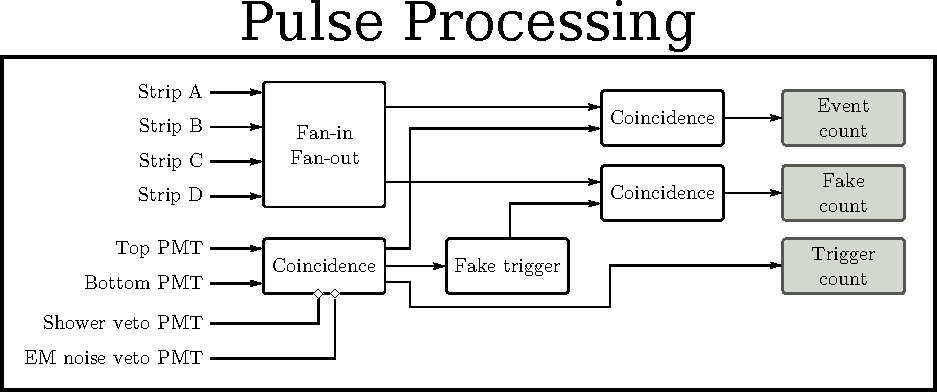
\includegraphics[width = 0.8\linewidth]{fig/chapt6/pulse-processing-2013.pdf}
			\caption{\label{fig:Pulse-Processing:C}}
		\end{subfigure}
		\caption{\label{fig:Pulse-Processing} The block diagrams corresponding to the signal treatment for both INFN preamplifier (Figure~\ref{fig:Pulse-Processing:A}) and CMS FEEs (Figure~\ref{fig:Pulse-Processing:B}) are shown. The digitized signals are then counted in coïncidence with the trigger signals provided by PMTs (Figure~\ref{fig:Pulse-Processing:C}).}
    \end{figure}
    
    The data taking program consisted in \acl{HV} scans. A first point was taken at \SI{0}{V} to only measure noise. Then the HV was increased to an applied value of \SI{7}{kV}. The voltage was increased in steps of \SI{500}{V} until \SI{8}{kV} from where it was increased in steps of \SI{100}{V} until an upper limit of \SI{10}{kV}. After rising the voltage over the electrodes of the RPC, a waiting period of 15 minutes was observed to leave time to the electrodes to charge and to the currents to stabilize. The currents were reported at the moment the data taking was started. At each HV step, except at \SI{0}{V}, approximatively 300 triggers were taken to estimate the efficiency of the detector by counting the number of hits in the system (A or B or C or D), referring to the strips. The noise rate per unit area was measured during the first \SI{100}{s} of data taking by counting the number of hits recieved in each read-out strip. The cluster size, the average number of adjacent strips fired during a muon event, could not be measured due to the lack of available scalers.
    
    During the data acquisition, in addition to counting the number of signals with respect to the number of triggers, the current or the noise rate per unit area as a function of the increasing voltage, the environmental parameters were monitored. Using the information provided by a humidity and temperature sensor on the gas input line together with the environmental pressure given by a weather station, the applied voltage could be corrected following Formula~\ref{eq:PTCMS}. Moreover, the voltage line was filtered to prevent noise and higher currents in the RPC under test.
    
    The results of the preliminary tests are presented in Figure~\ref{fig:INFN-preamp}. More details on the performance shift are provided in Table~\ref{tab:INFN-preamp}. Being able to use electronics with a much higher sensitivity allows for a HV shift of up to \SI{475}{V} with a threshold as low as \SI{3}{fC} corresponding to the lowest threshold available on the discriminator modules used in the experiment. Indeed, the NIM quad discriminator 821 manufactured by LECROY only allows at minimum to set the threshold at a voltage of approximately \SI{30}{mV} on the input signals. Thus, two values of discrimination were used ($\sim$\SI{75}{mV} and $\sim$\SI{30}{mV}).
	
	\begin{figure}[H]
		\begin{subfigure}{.5\linewidth}
		    \centering
			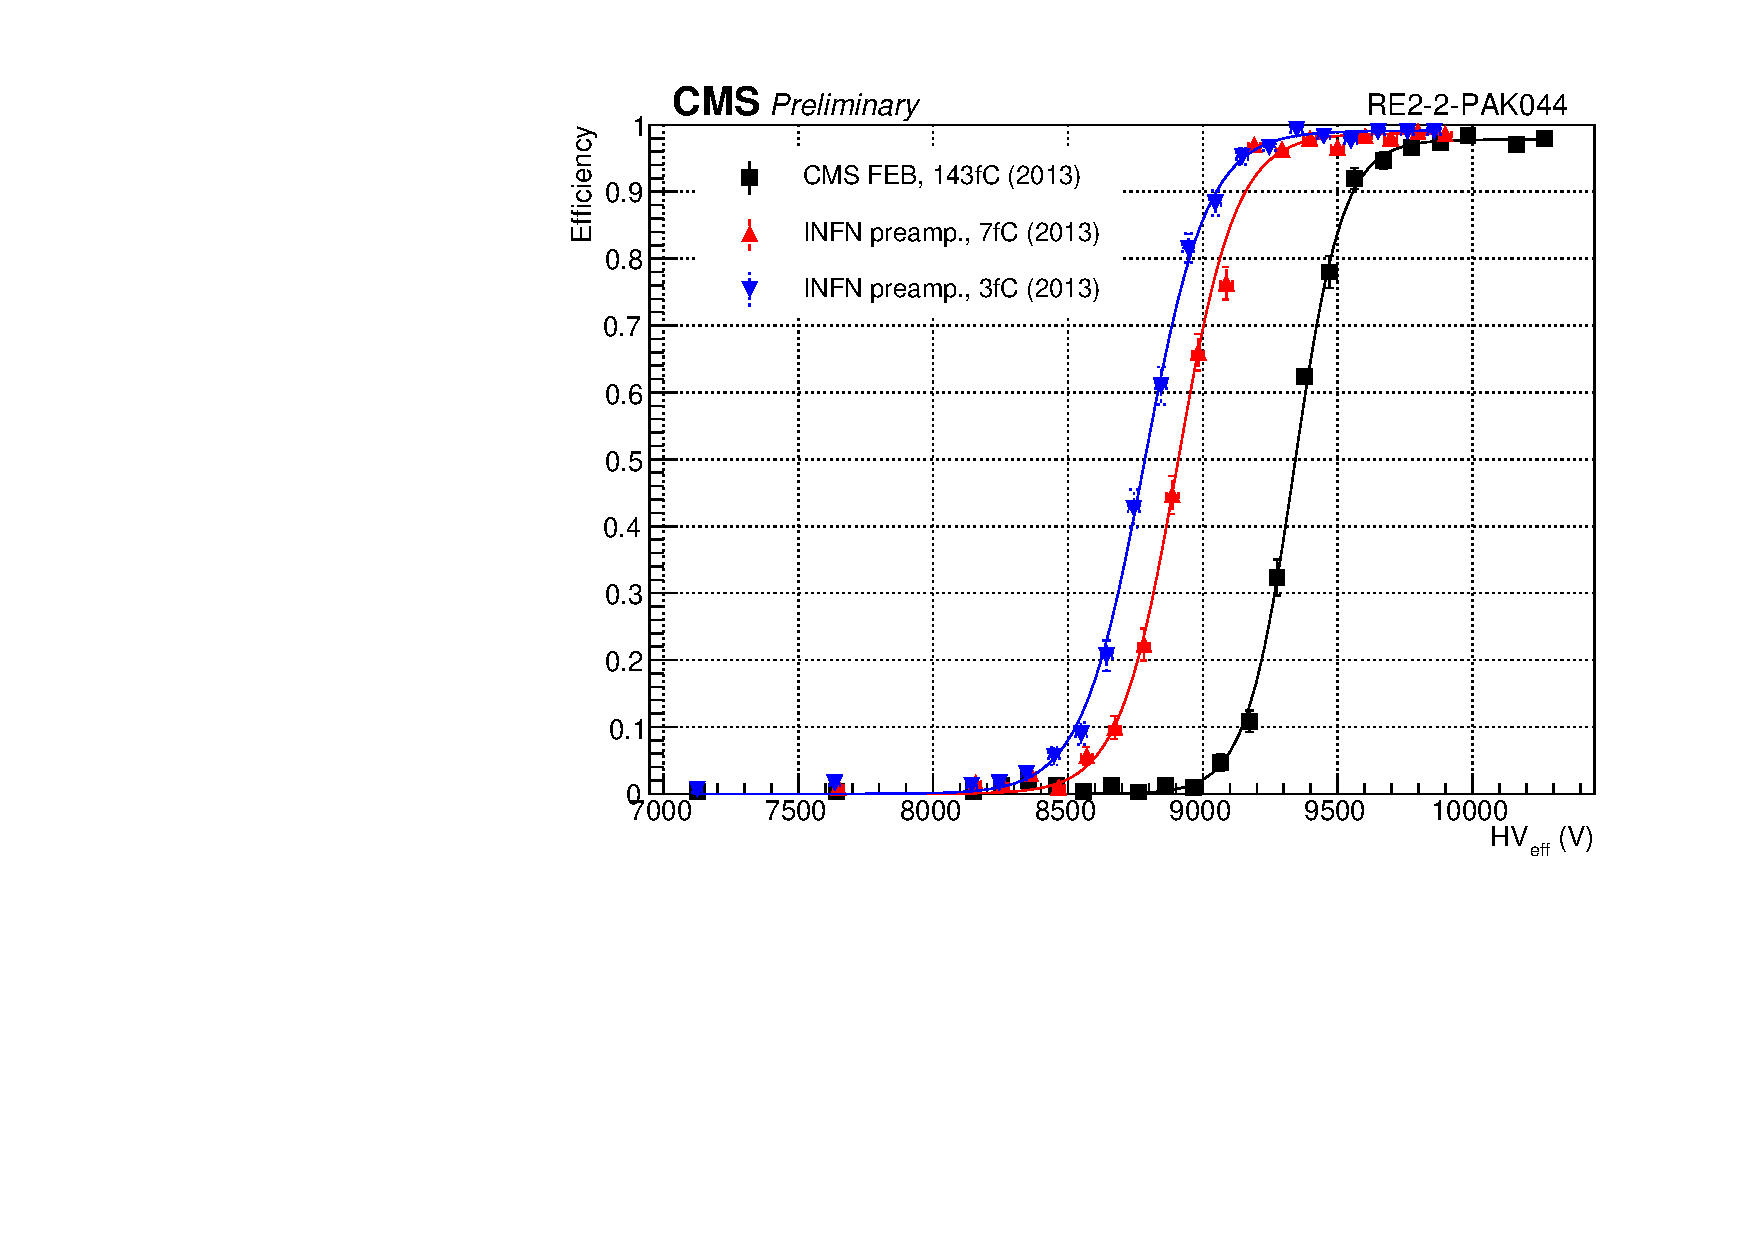
\includegraphics[width=\linewidth]{fig/chapt6/INFN-Preamplifier-Shift.pdf}
			\caption{\label{fig:INFN-preamp:A}}
		\end{subfigure}
		\begin{subfigure}{.5\linewidth}
		    \centering
			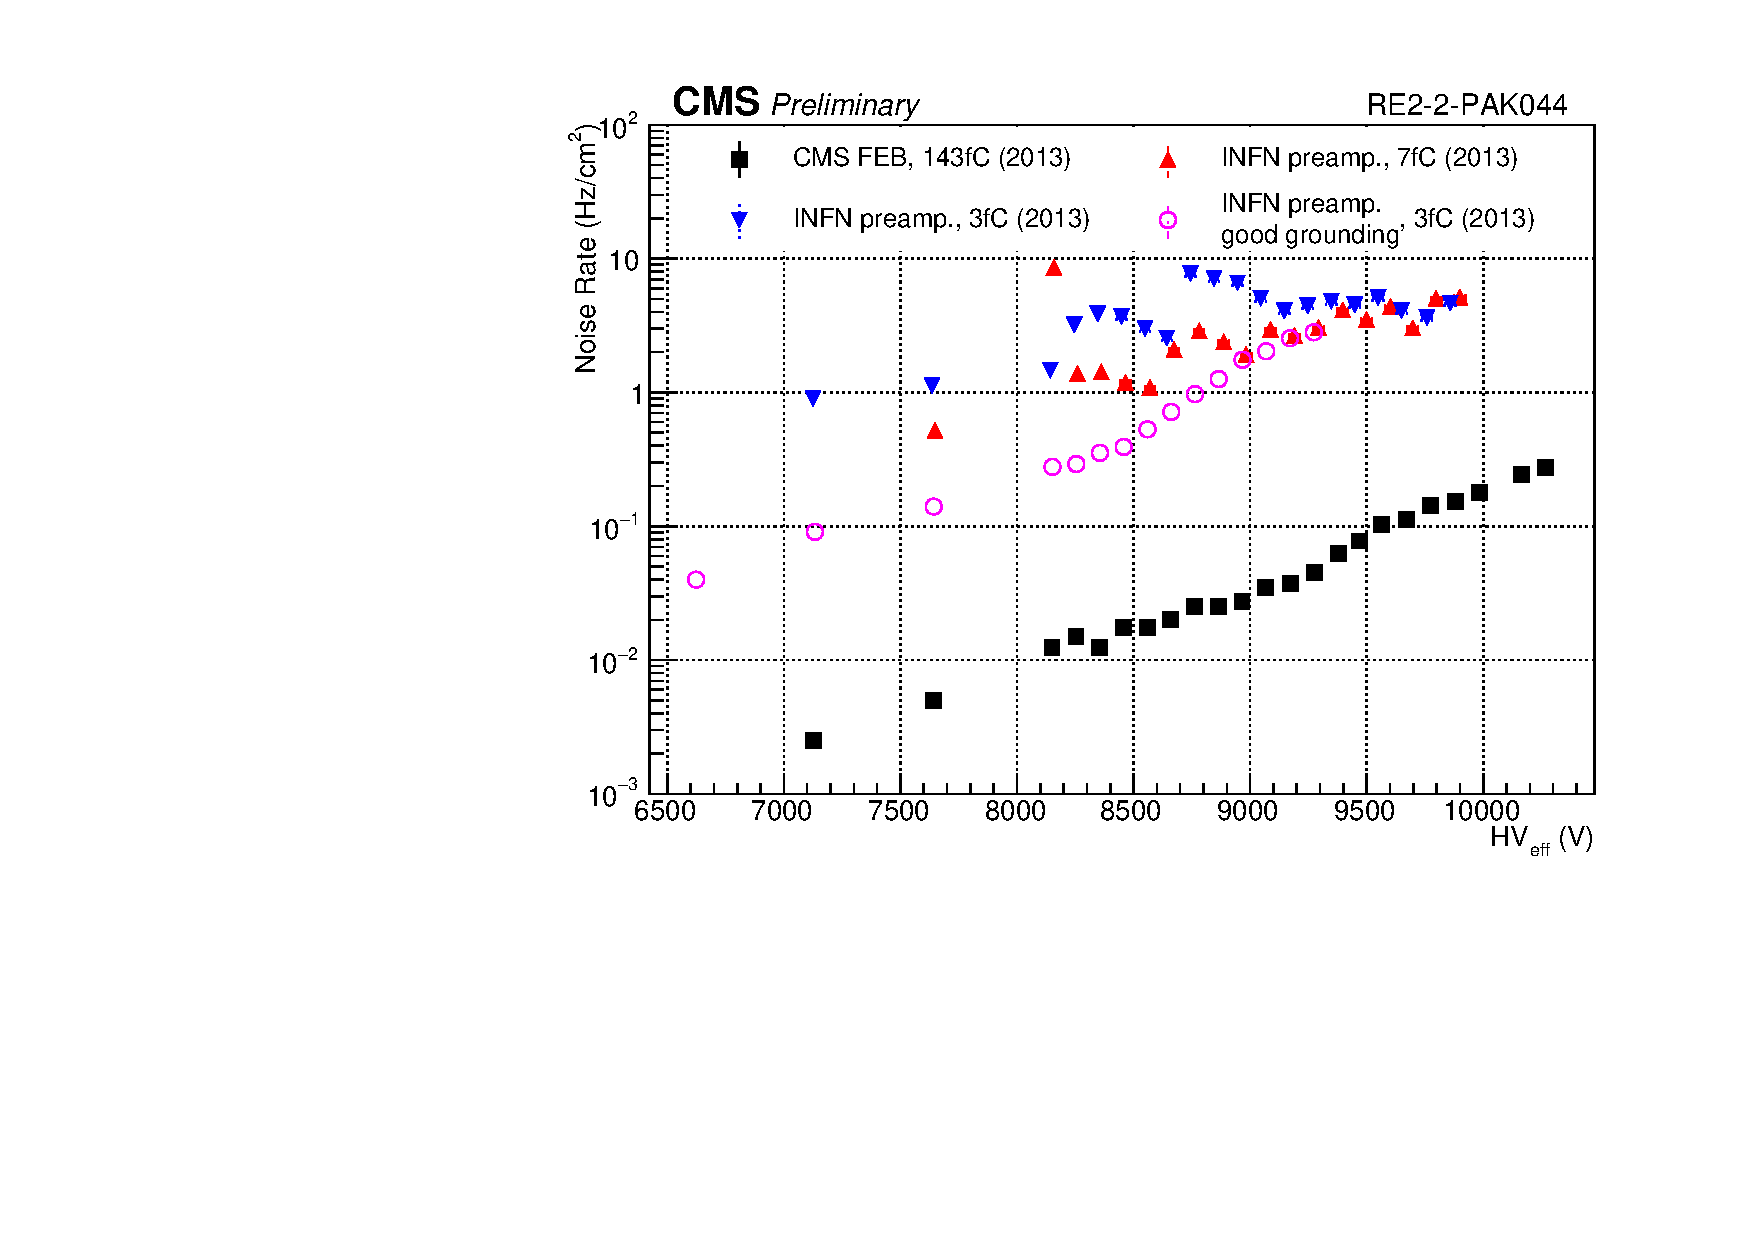
\includegraphics[width = \linewidth]{fig/chapt6/INFN-Preamplifier-Rate-Shift.pdf}
			\caption{\label{fig:INFN-preamp:B}}
		\end{subfigure}
		\caption{\label{fig:INFN-preamp} Efficiency (Figure~\ref{fig:INFN-preamp:A}) and noise rate per unit area (Figure~\ref{fig:INFN-preamp:B}) of the CMS RE2-2 detector tested with the standard CMS FEBs (black) and with the INFN preamplifier at different thresholds (red and blue).}
	\end{figure}
	
	\begin{table}[H]
		\caption{\label{tab:INFN-preamp} Results of the sigmoid fit (Formula~\ref{eq:Sigmoid}) performed on the data presented in Figure~\ref{fig:INFN-preamp:A}. The working point and its corresponding efficiency are computed using Formula~\ref{eq:KneeWP}.}
		\footnotesize
		\begin{tabular}{|c|c|c|c|c|c|}
			\hline
			Data & $\epsilon_{max}$ & $\lambda$ ($\times$\Ord{-2} \si{V^{-1}}) & $HV_{50}$ (\si{V}) & $\epsilon_{WP}$ & $HV_{WP}$ (\si{V}) \\ 
			\hline
			CMS FEB, 156fC (2013) & \numerror{0.978}{0.004} & \numerror{1.12}{0.07} & \numerror{9339}{11} & \numerror{0.97}{0.01} & \numerror{9752}{27}\\ 
			\hline
			INFN preamp., 7fC (2013) & \numerror{0.987}{0.003} & \numerror{0.93}{0.05} & \numerror{8907}{11} & \numerror{0.97}{0.01} & \numerror{9374}{27}\\ 
			\hline
			INFN preamp., 3fC (2013) & \numerror{0.991}{0.003} & \numerror{0.86}{0.04} & \numerror{8783}{11} & \numerror{0.98}{0.01} & \numerror{9276}{27}\\ 
			\hline
		\end{tabular}
	\end{table}

	\subsection{INFN preamplifiers mounted onto CMS \acl{FEB}}
	\label{chapt6:ssec:INFN-FEB}
	
	Following the first experiment performed in the experimental hall aside of the old GIF, a new series of tests has been done in the CMS RPC assembly laboratory at CERN. For this purpose, the preamplifiers have been designed to be standalone single channels. To have a consistent comparison with the CMS FEB, a FEB prototype has been built based on the current CMS design. As shown in Figure~\ref{fig:Setup-INFN-904}, the preamplifiers are meant to be plugged in one of the available 16 channels of the board that produces an LVDS output with similar characteristics than the CMS FEB.
	 
	\begin{figure}[H]
		\begin{subfigure}{.5\linewidth}
		    \centering
			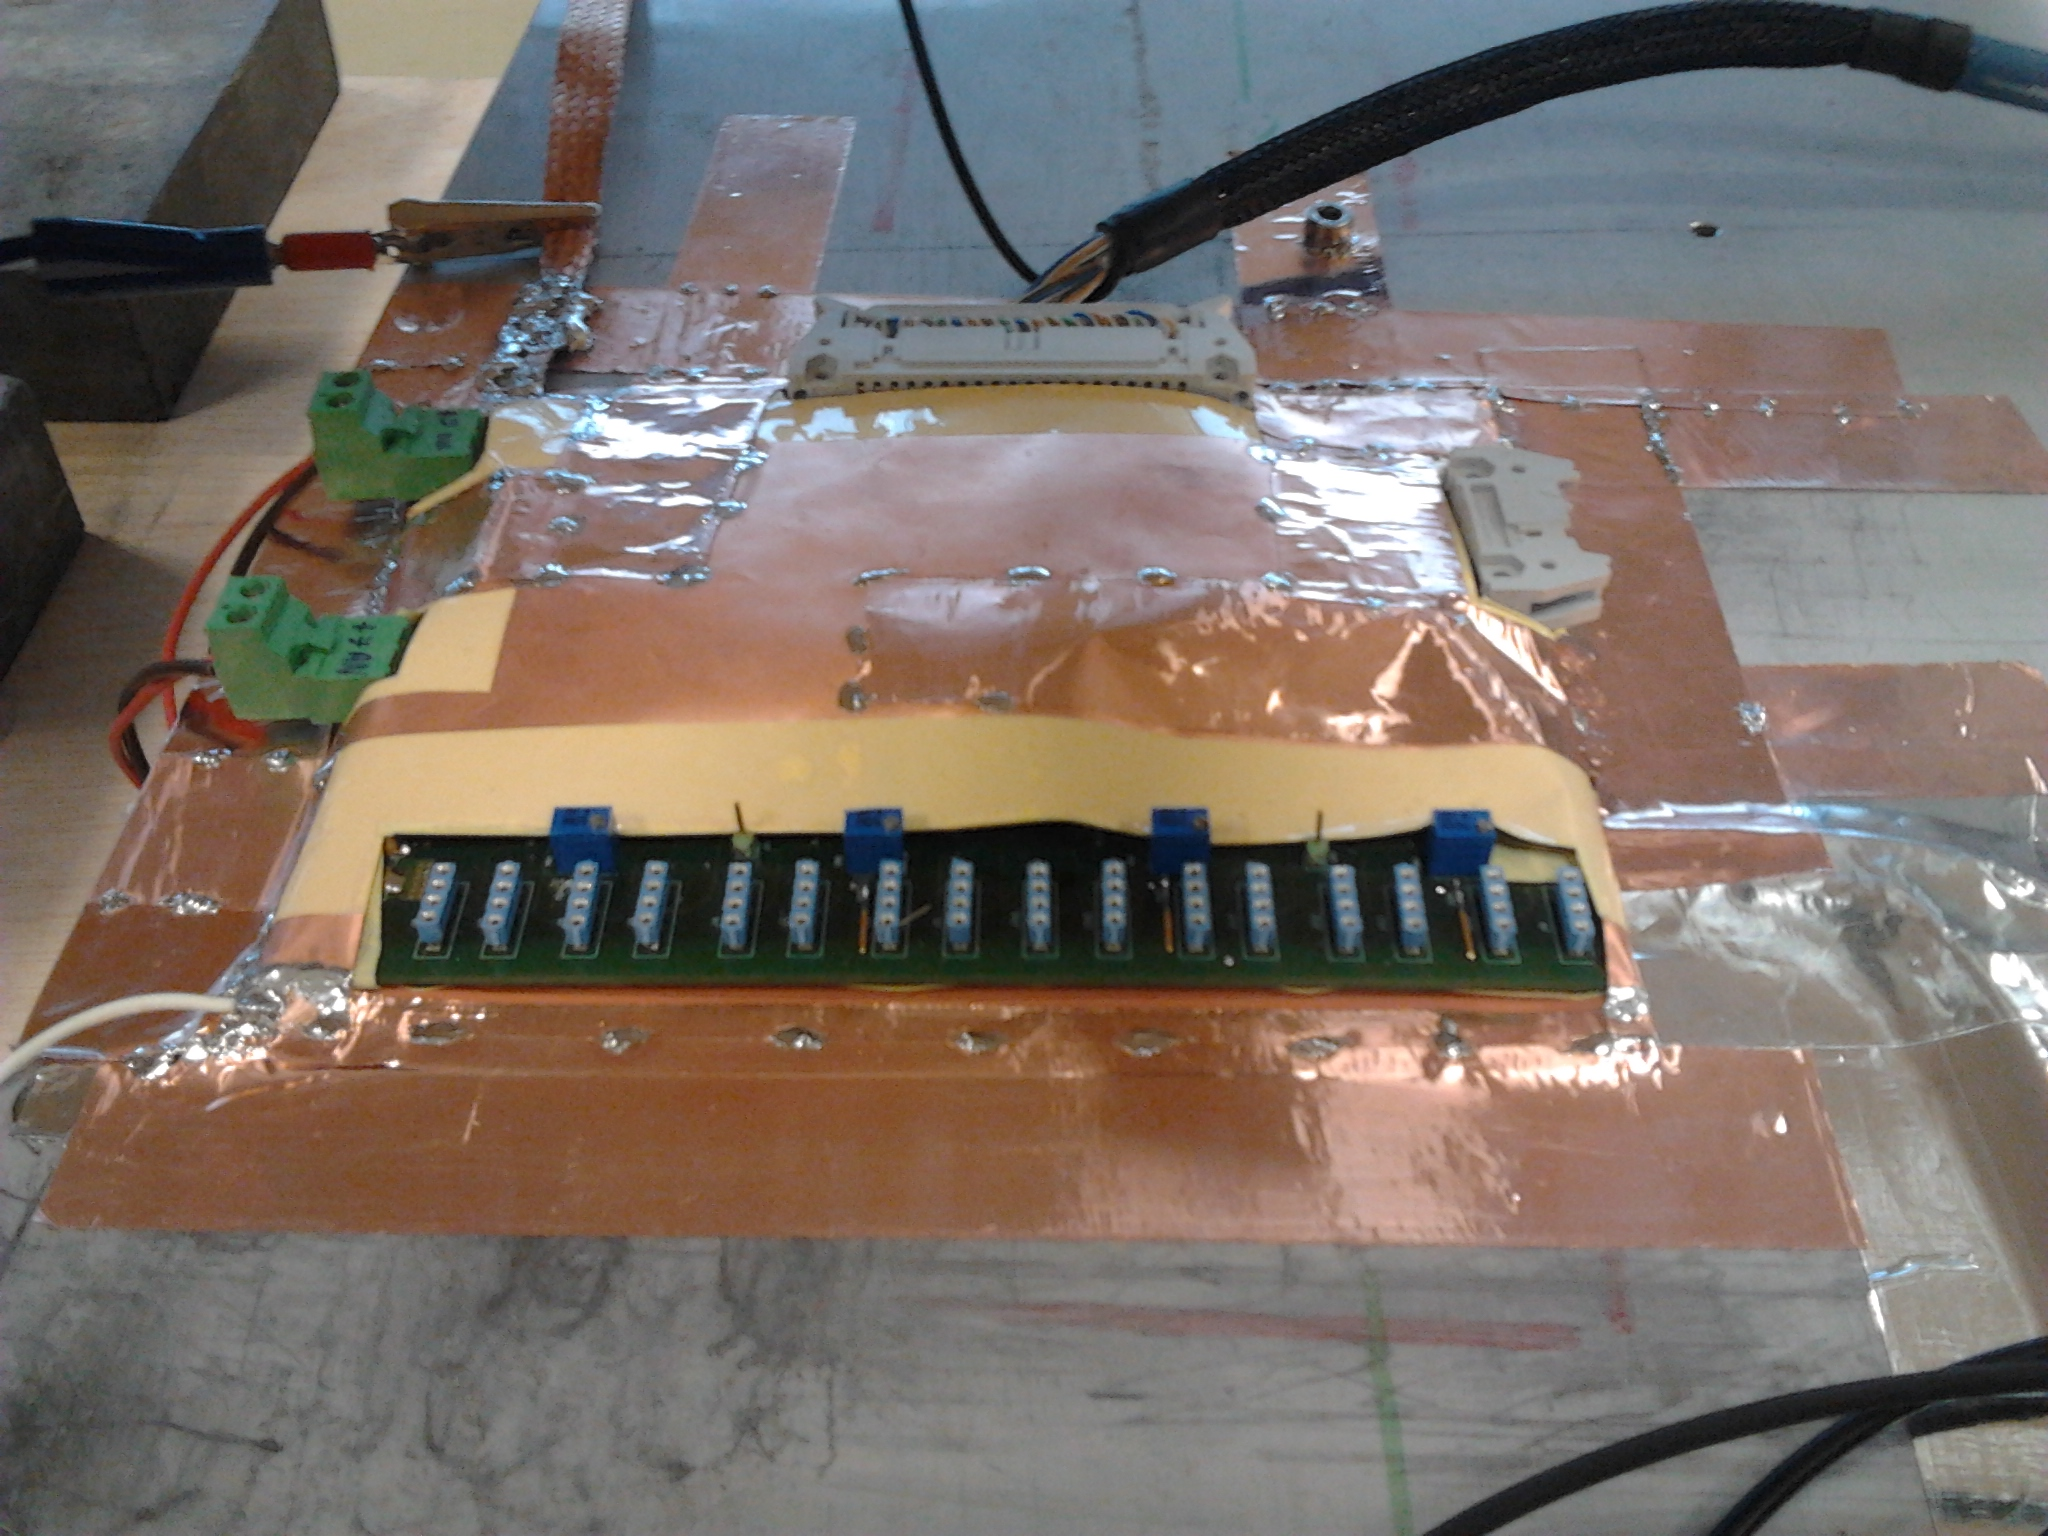
\includegraphics[width = \linewidth]{fig/chapt6/ATLAS_FEB.png}
			\caption{\label{fig:Setup-INFN-904:A}}
		\end{subfigure}
		\begin{subfigure}{.5\linewidth}
		    \centering
			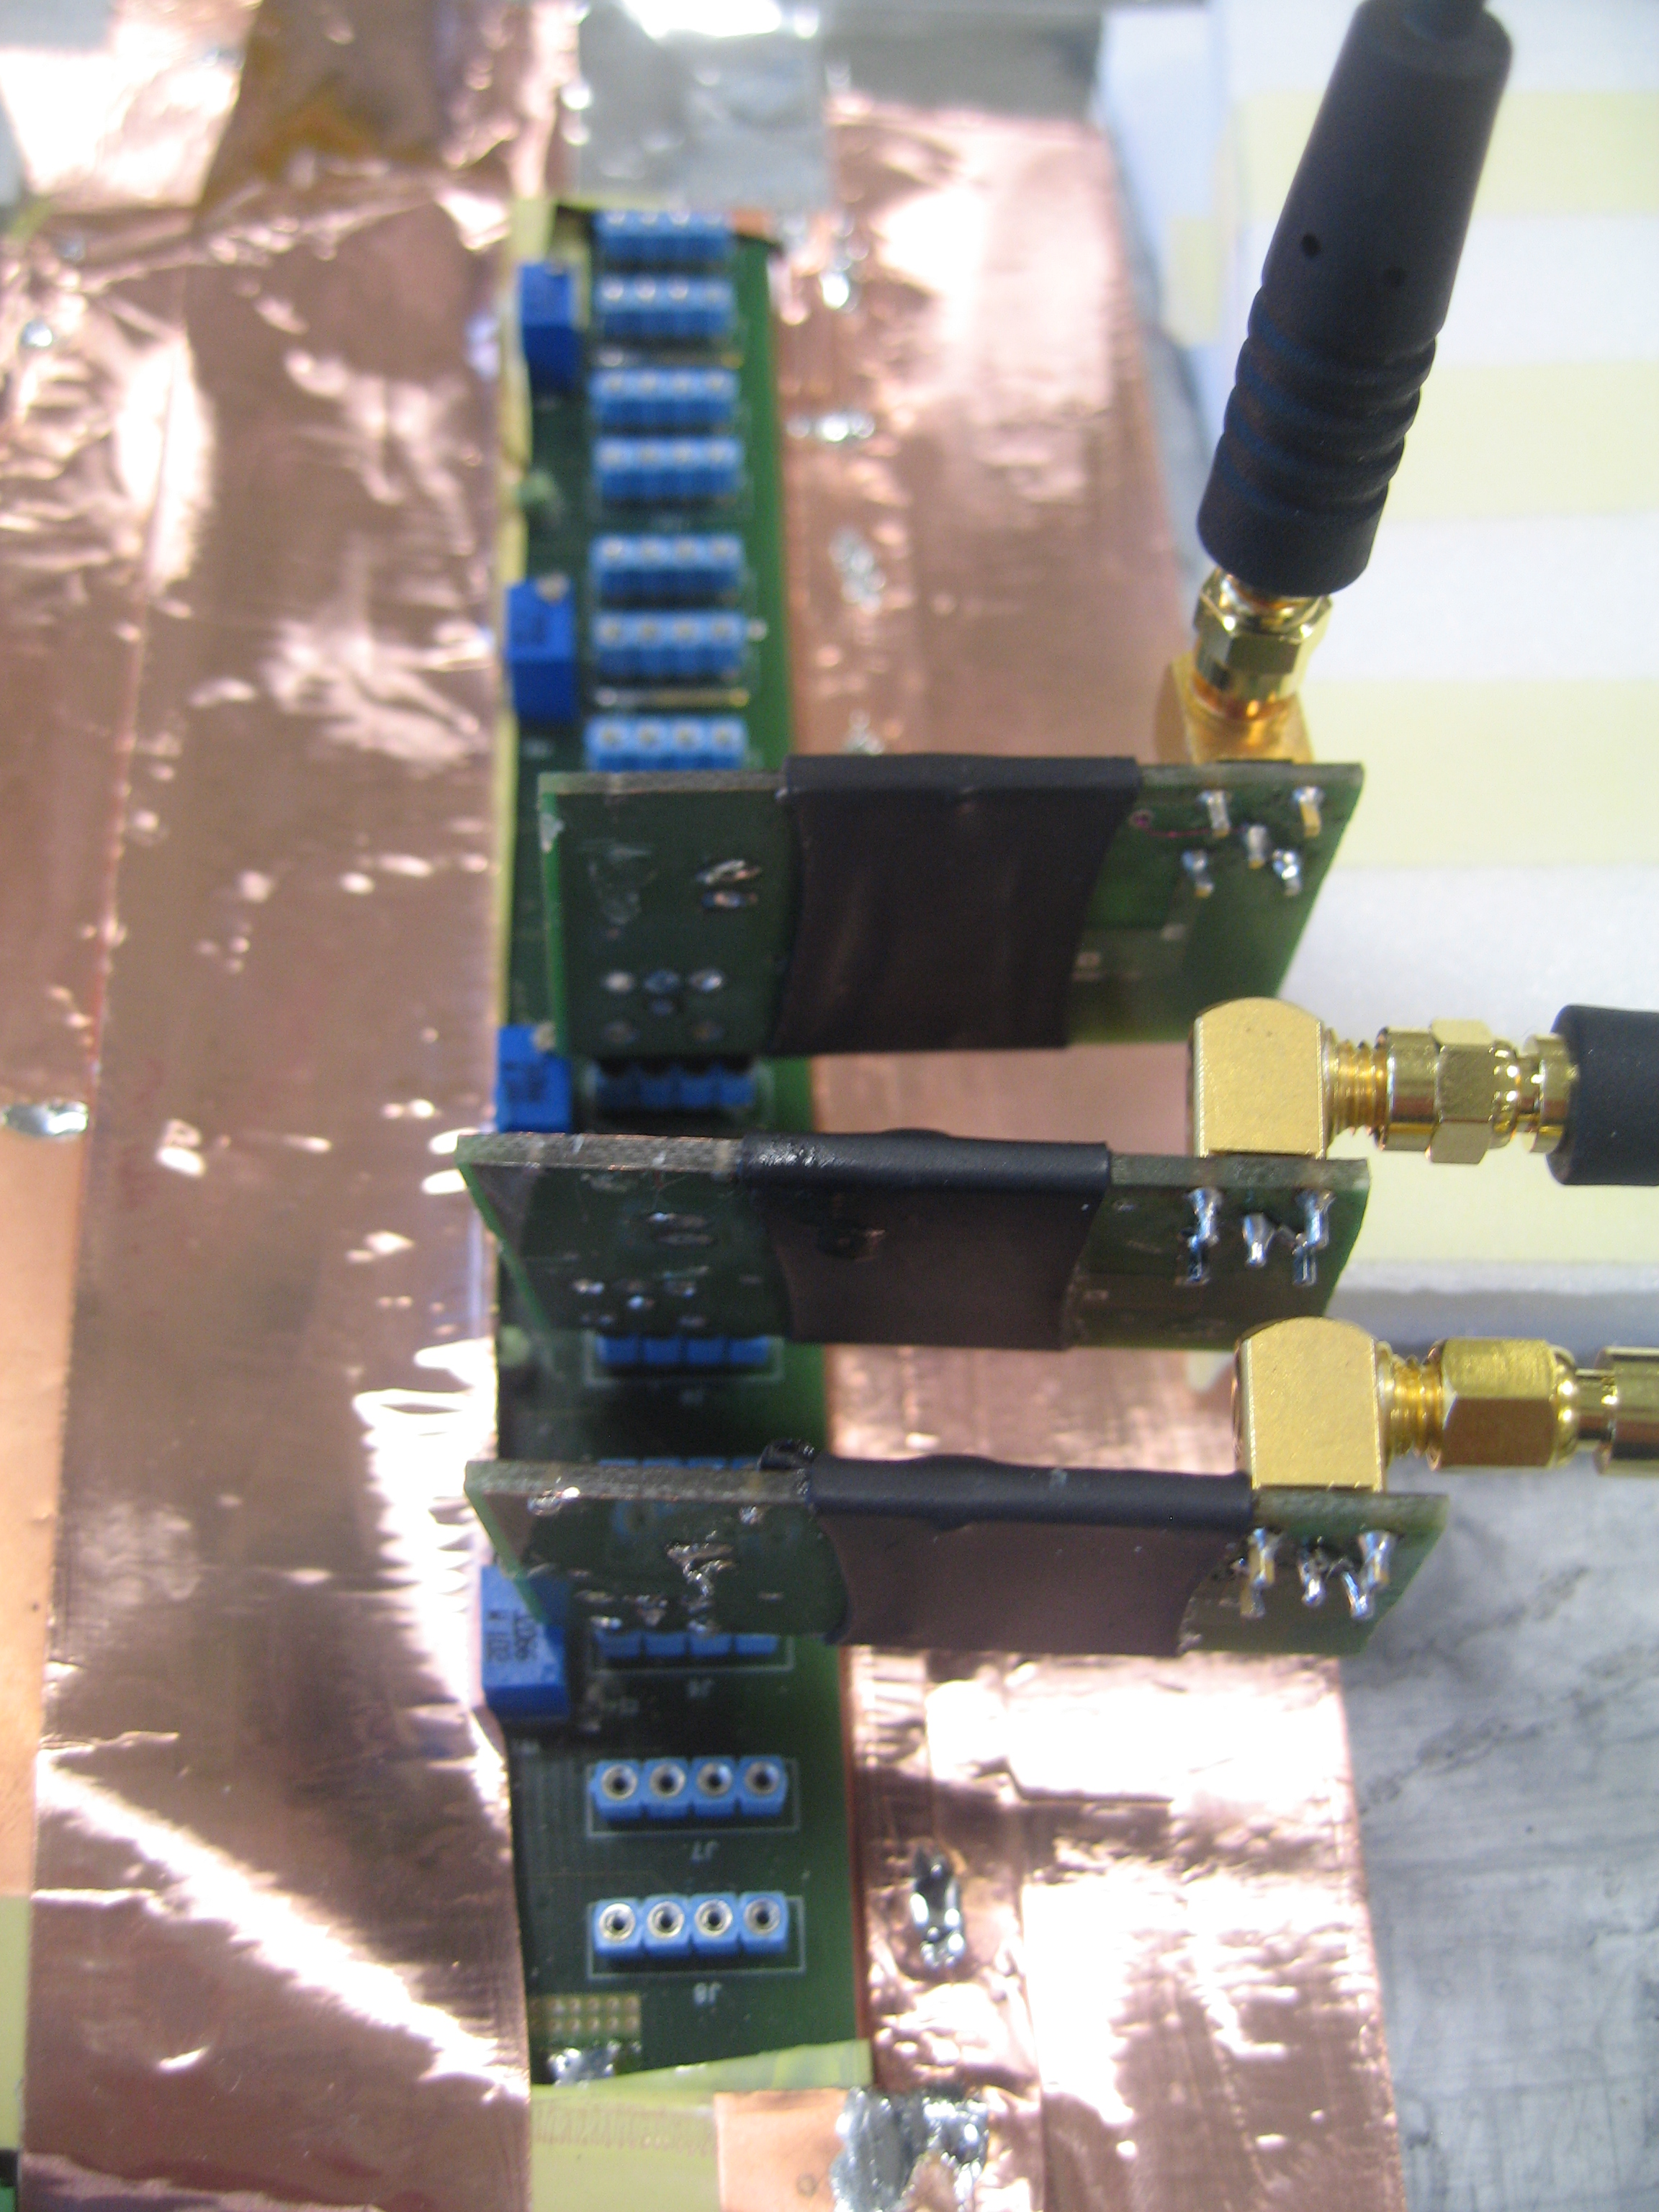
\includegraphics[width = 0.56\linewidth]{fig/chapt6/ATLAS_preamp.JPG}
			\caption{\label{fig:Setup-INFN-904:B}}
		\end{subfigure}
		\begin{subfigure}{\linewidth}
		    \centering
			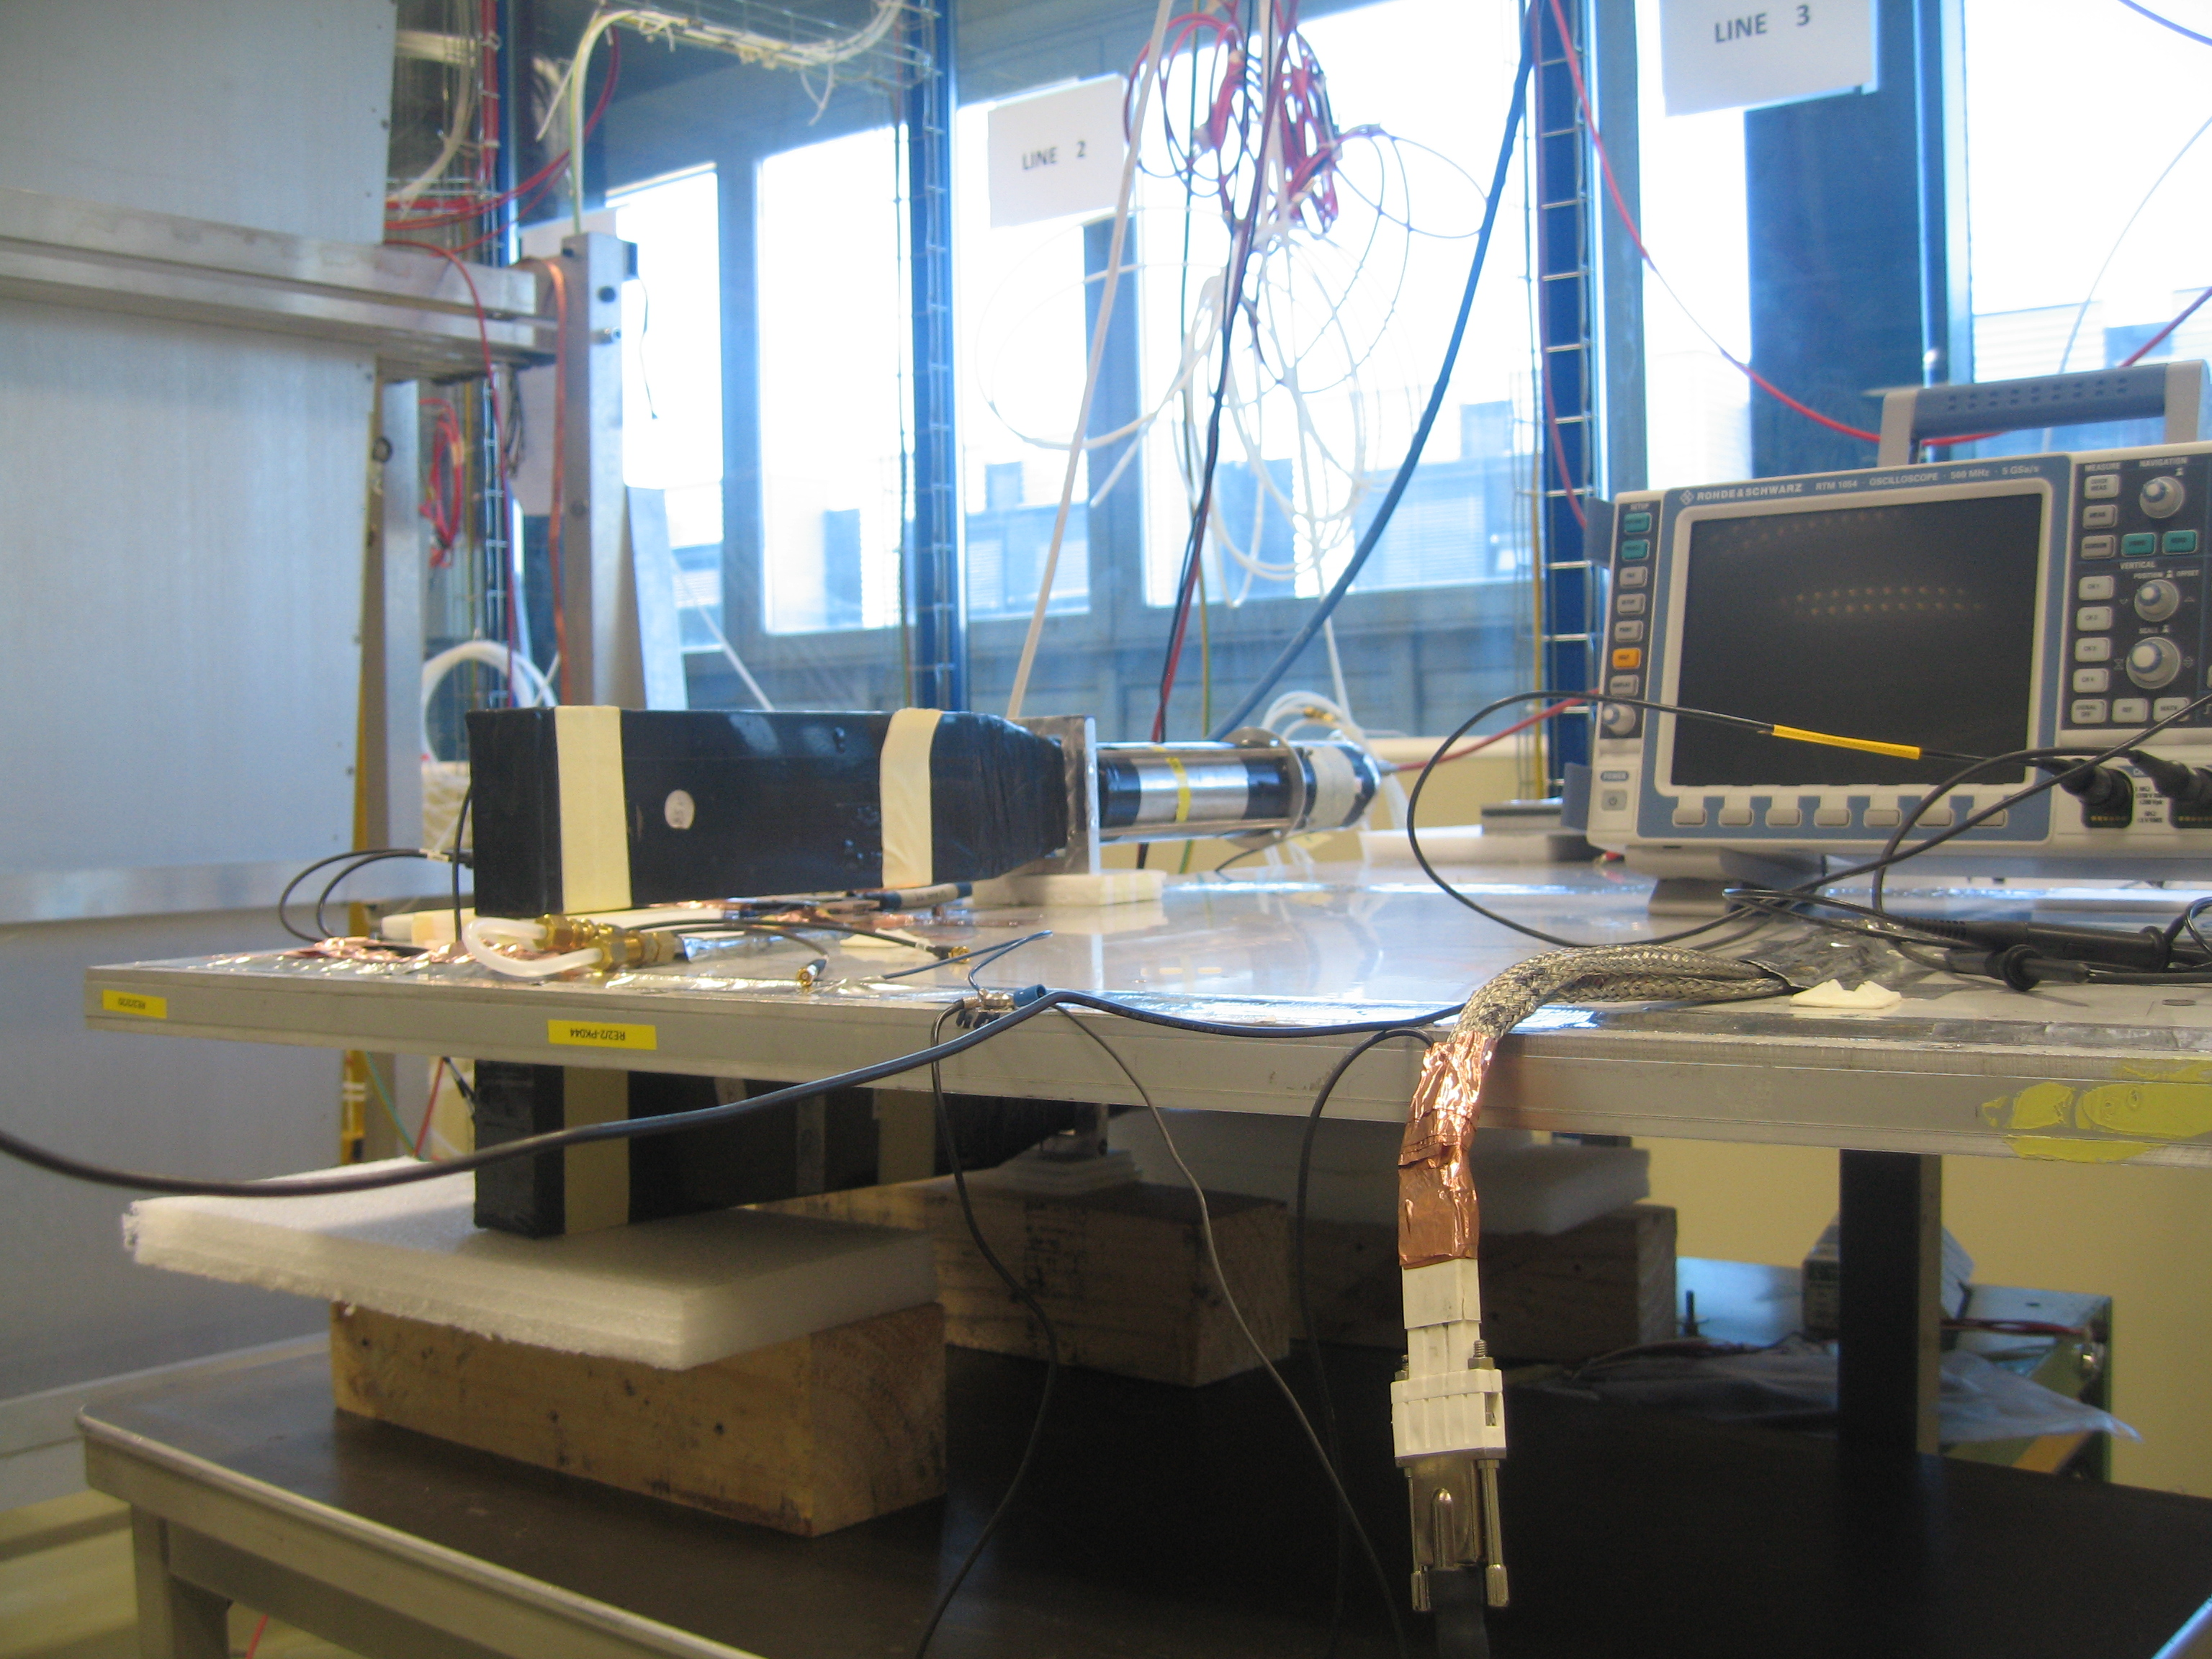
\includegraphics[width = 0.5\linewidth]{fig/chapt6/Setup_ATLAS_PAK.JPG}
			\caption{\label{fig:Setup-INFN-904:C}}
		\end{subfigure}
		\caption{\label{fig:Setup-INFN-904} Figure~ref{fig:Setup-INFN-904:A}: Shielded \acl{FEB} on which the INFN preamplifiers are to be mounted. Figure~ref{fig:Setup-INFN-904:B}: Three INFN preamplifiers connected onto the test FEB. Figure~ref{fig:Setup-INFN-904:C}: Experimental setup used to test the INFN preamplifier single mounted on a FEB similar to the CMS FEB.}
    \end{figure}
	
	At the time of the second experiment, only three channels could be lended by the team of INFN Roma. It was then decided to use the same PMTs than in the first measurements as trigger. This time, they were placed on their side to only cover an area on the detector smaller than three strips. On the data acquisition side, no DAQ software was available yet at the time of experimentation and scalers were once again used. As can be seen from Figure~\ref{Pulse-Processing-904}, the pulse processing has been inspired by the one used in the first experiment. Thanks to the lower number of channels to monitor, the cluster size could be estimated by counting the signals on single channels but also on groups of two and three channels in coincidence with the trigger.
	
	\begin{figure}[H]
		\centering
		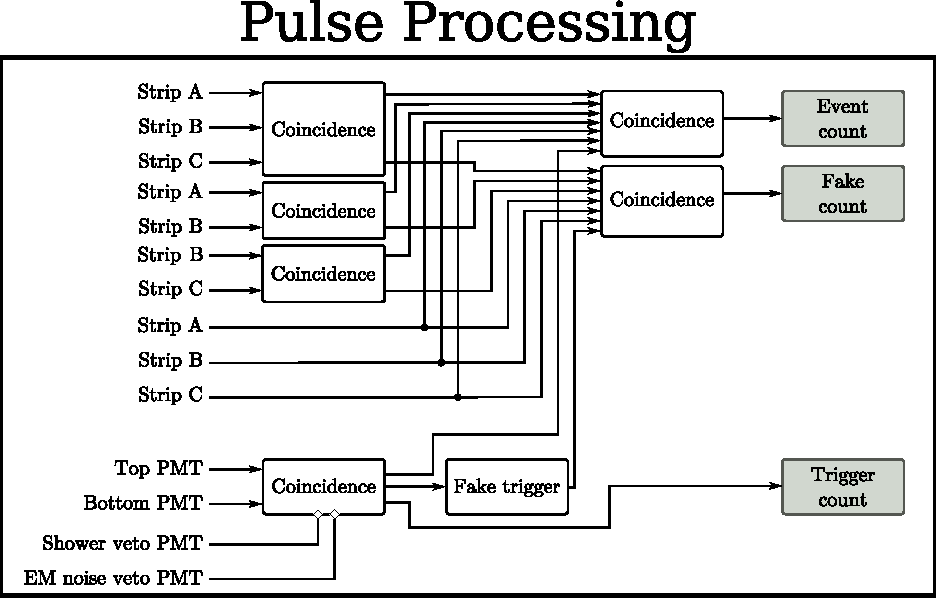
\includegraphics[width=.8\linewidth]{fig/chapt6/pulse-processing-2014.pdf}
		\caption{\label{fig:fig:Pulse-Processing-904} Similarly to Figure~\ref{fig:Pulse-Processing:C}, the signals are then counted in coïncidence with the trigger signals provided by PMTs. To estimate the cluster size, the channels are counted by groups of three, two and alone.}
	\end{figure}
	
	\begin{figure}[H]
		\begin{subfigure}{.5\linewidth}
		    \centering
			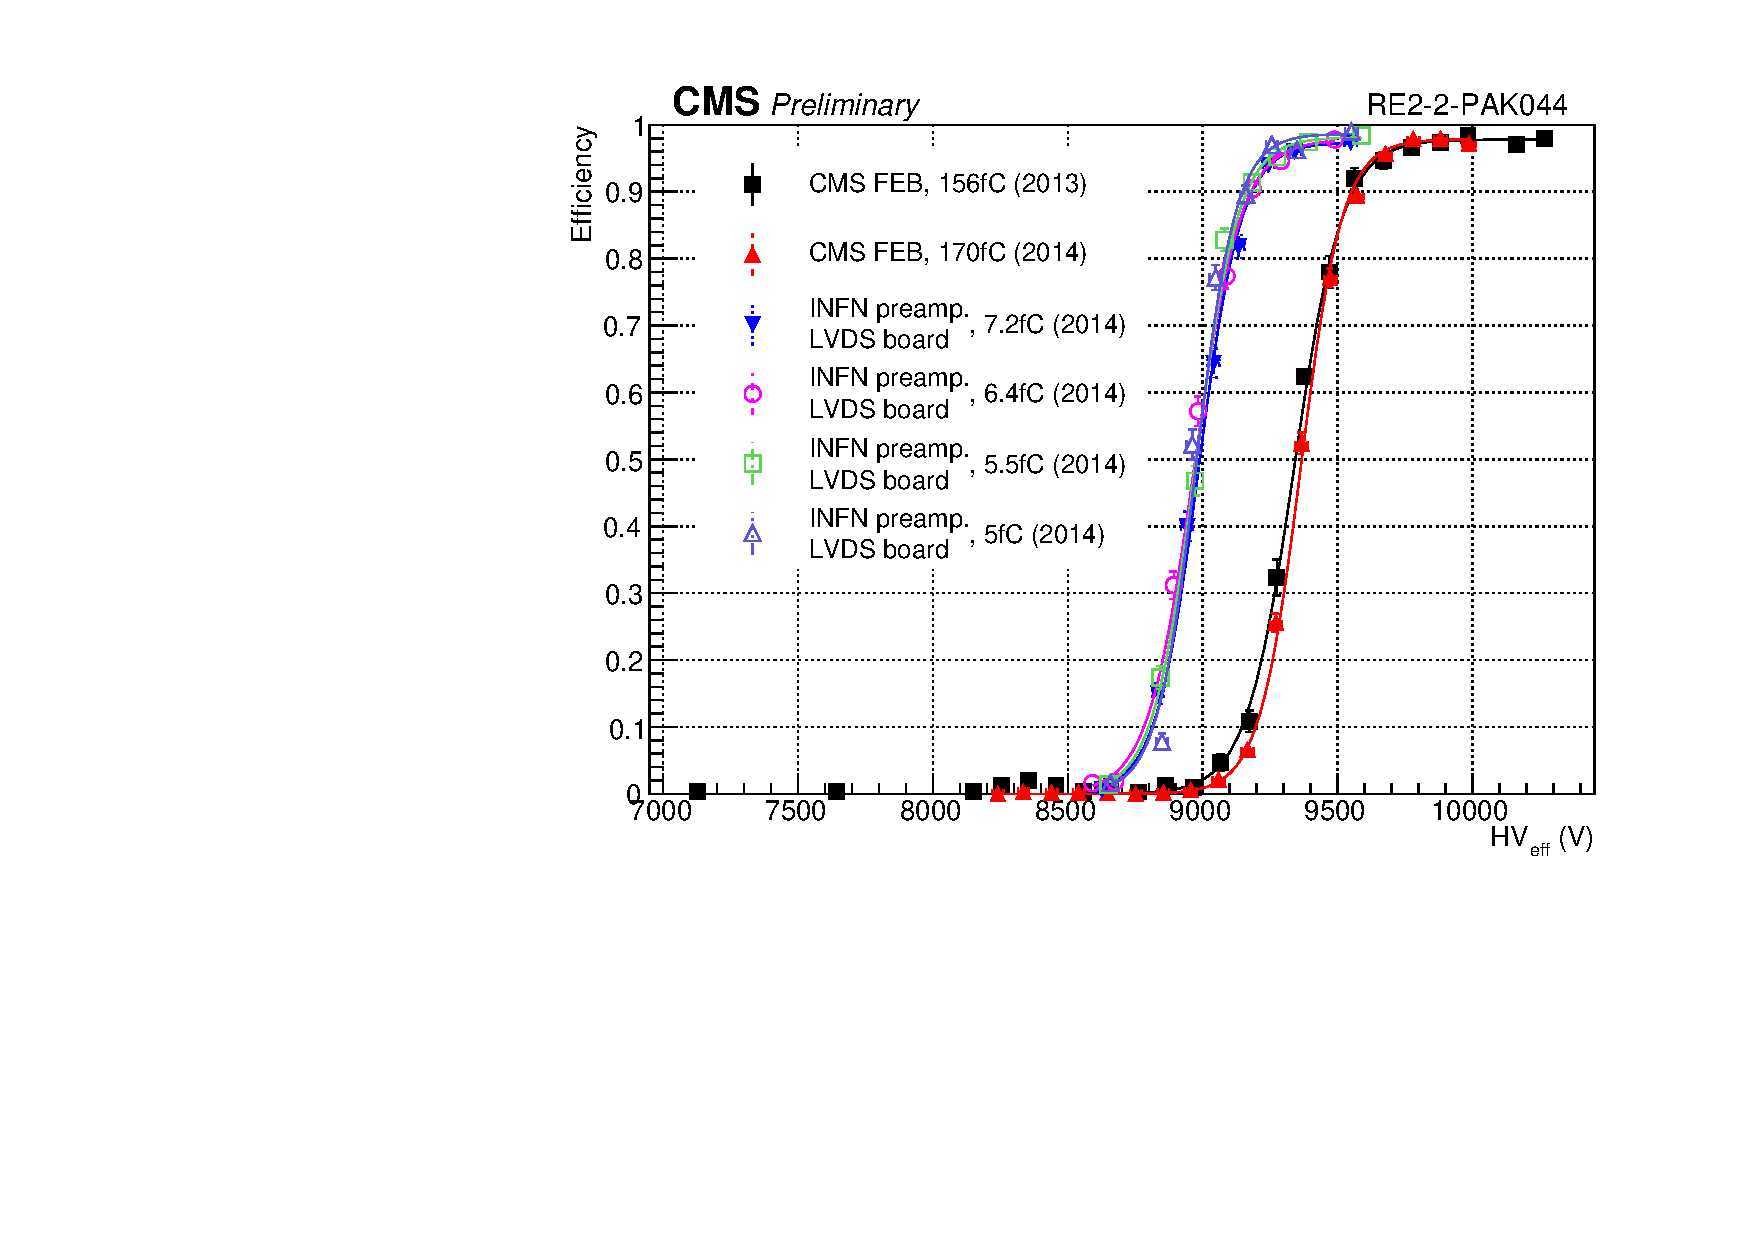
\includegraphics[width=\linewidth]{fig/chapt6/INFN-LVDS-Eff-Shift.pdf}
			\caption{\label{fig:INFN-FEB:A}}
		\end{subfigure}
		\begin{subfigure}{.5\linewidth}
		    \centering
			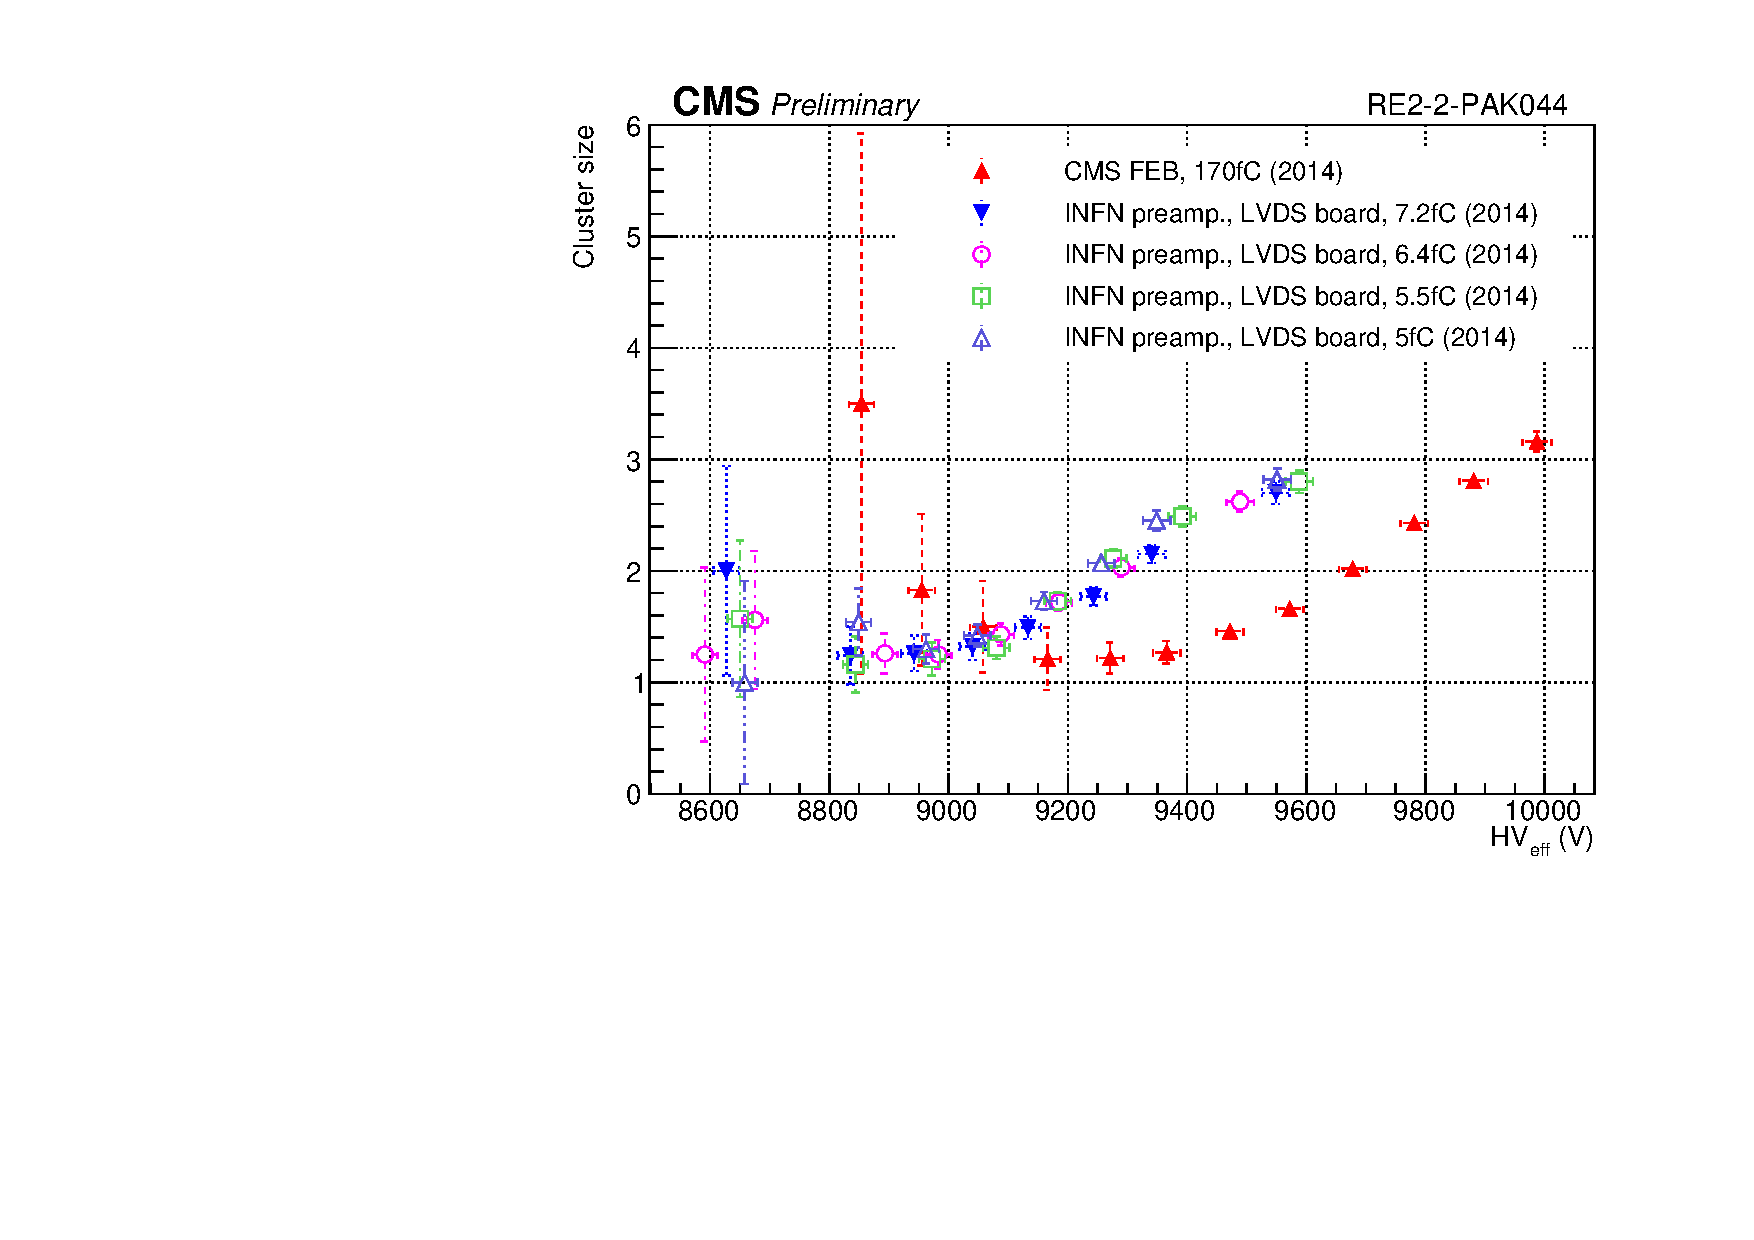
\includegraphics[width = \linewidth]{fig/chapt6/INFN-LVDS-ClS-Shift.pdf}
			\caption{\label{fig:INFN-FEB:B}}
		\end{subfigure}
		\begin{subfigure}{\linewidth}
		    \centering
			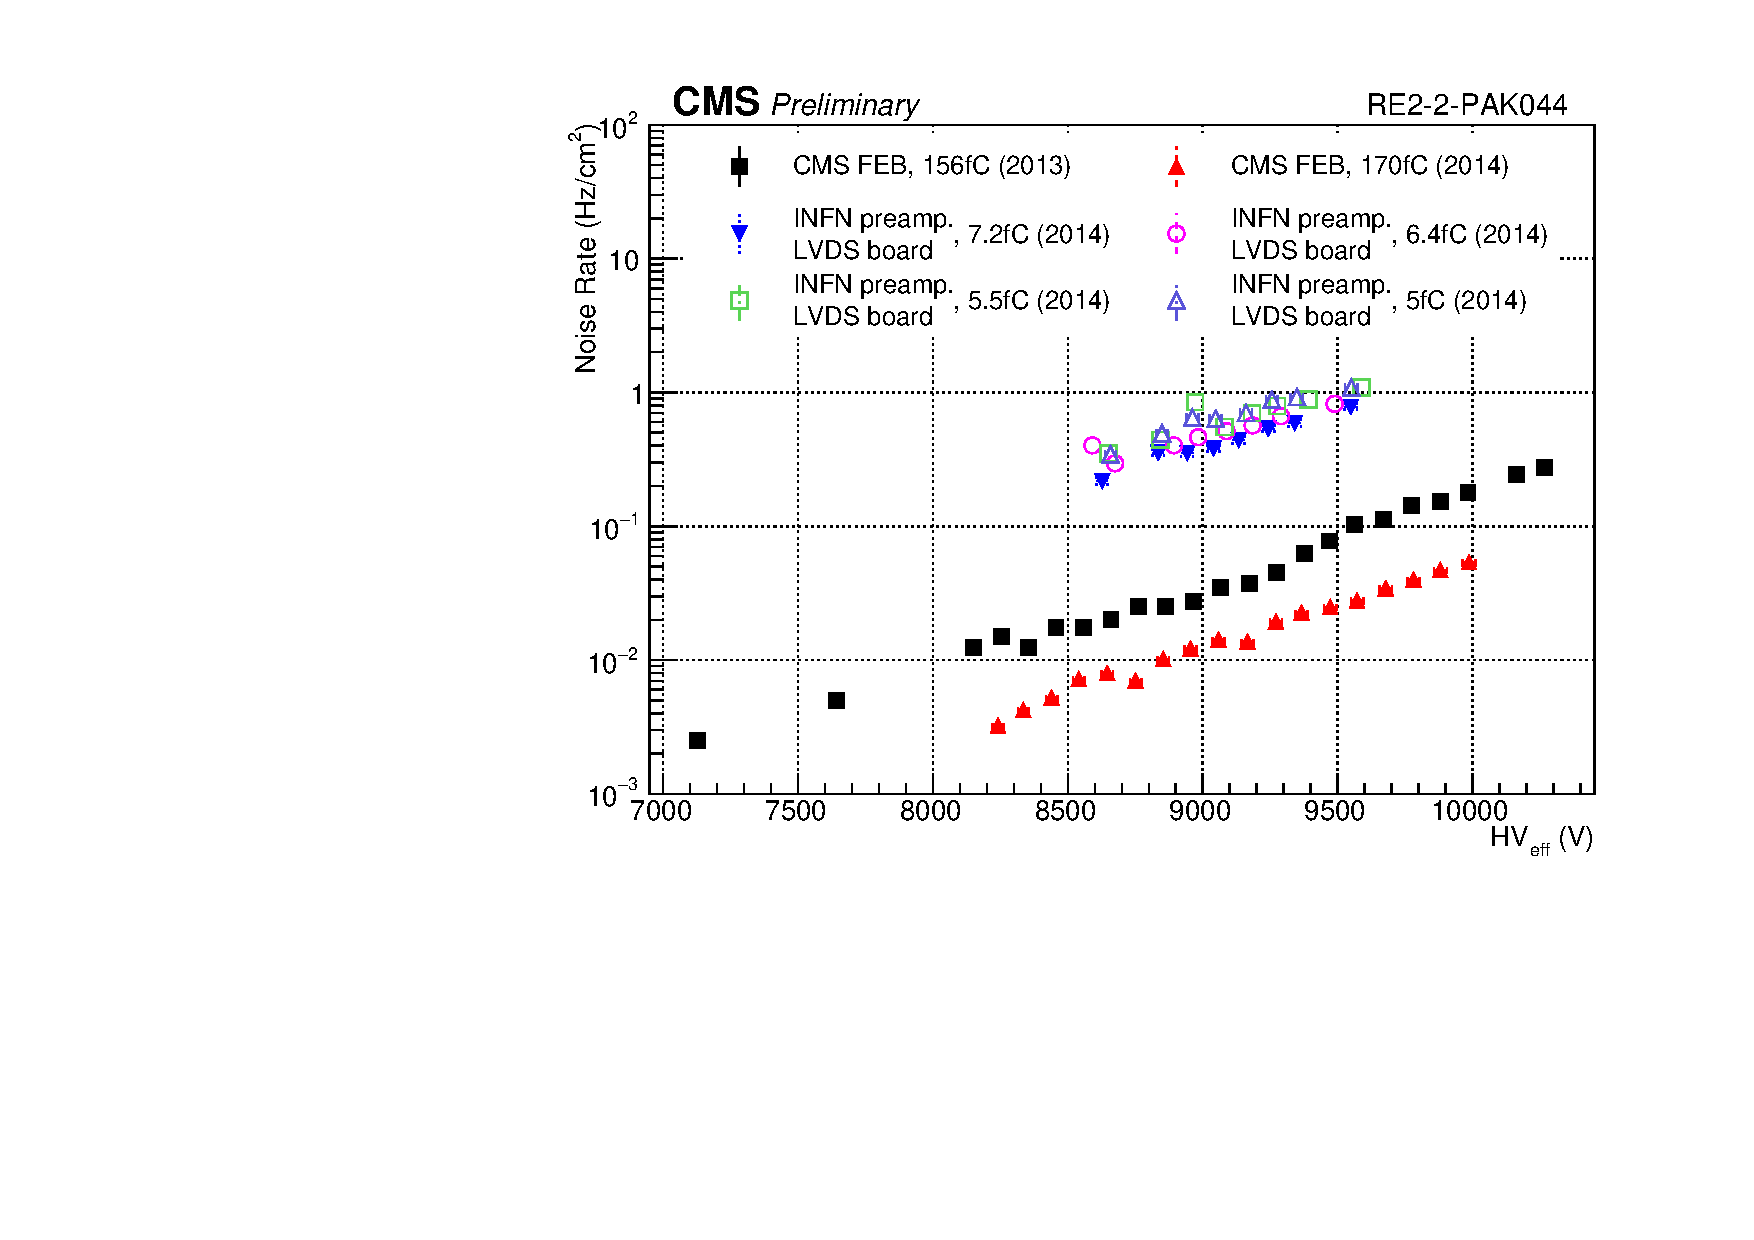
\includegraphics[width = .5\linewidth]{fig/chapt6/INFN-LVDS-Rate-Shift.pdf}
			\caption{\label{fig:INFN-FEB:C}}
		\end{subfigure}
		\caption{\label{fig:INFN-FEB} Efficiency (Figure~\ref{fig:INFN-FEB:A}), cluster size (Figure~\ref{fig:INFN-FEB:B}) and noise rate per unit area (Figure~\ref{fig:INFN-FEB:C}) of the CMS RE2-2 detector tested with the standard CMS FEBs (black) and with the INFN preamplifier mounted onto the CMS FEB at different thresholds (red, blue, pink, green and purple).}
	\end{figure}
	
	\begin{table}[H]
		\caption{\label{tab:INFN-FEB} Results of the sigmoid fit (Formula~\ref{eq:Sigmoid}) performed on the data presented in Figure~\ref{fig:INFN-FEB:A}. The working point and its corresponding efficiency are computed using Formula~\ref{eq:KneeWP}.}
		\footnotesize
		\begin{tabular}{|c|c|c|c|c|c|}
			\hline
			Data & $\epsilon_{max}$ & $\lambda$ ($\cdot$\Ord{-2} \si{V^{-1}}) & $HV_{50}$ (\si{V}) & $\epsilon_{WP}$ & $HV_{WP}$ (\si{V}) \\ 
			\hline
			CMS FEB, 156fC (2013) & \numerror{0.978}{0.004} & \numerror{1.12}{0.07} & \numerror{9339}{11} & \numerror{0.97}{0.01} & \numerror{9752}{27}\\ 
			\hline
			CMS FEB, 170fC (2014) & \numerror{0.978}{0.003} & \numerror{1.30}{0.06} & \numerror{9364}{9} & \numerror{0.97}{0.01} & \numerror{9740}{19}\\ 
			\hline
			INFN/CMS FEB, 7.2fC (2014) & \numerror{0.973}{0.006} & \numerror{1.26}{0.09} & \numerror{8985}{10} & \numerror{0.97}{0.01} & \numerror{9368}{26}\\ 
			\hline
			INFN/CMS FEB, 6.4fC (2014) & \numerror{0.978}{0.007} & \numerror{1.16}{0.08} & \numerror{8969}{11} & \numerror{0.97}{0.01} & \numerror{9372}{28}\\ 
			\hline
			INFN/CMS FEB, 5.5fC (2014) & \numerror{0.981}{0.005} & \numerror{1.26}{0.09} & \numerror{8973}{12} & \numerror{0.97}{0.01} & \numerror{9357}{28}\\ 
			\hline
			INFN/CMS FEB, 5fC (2014) & \numerror{0.987}{0.004} & \numerror{1.37}{0.10} & \numerror{8976}{12} & \numerror{0.98}{0.01} & \numerror{9342}{28}\\ 
			\hline
		\end{tabular}
	\end{table}

	\subsection{HARDROC 2 readout panel}
	\label{chapt6:ssec:HARDROC2}
	 
	\begin{figure}[H]
		\begin{subfigure}{.5\linewidth}
		    \centering
			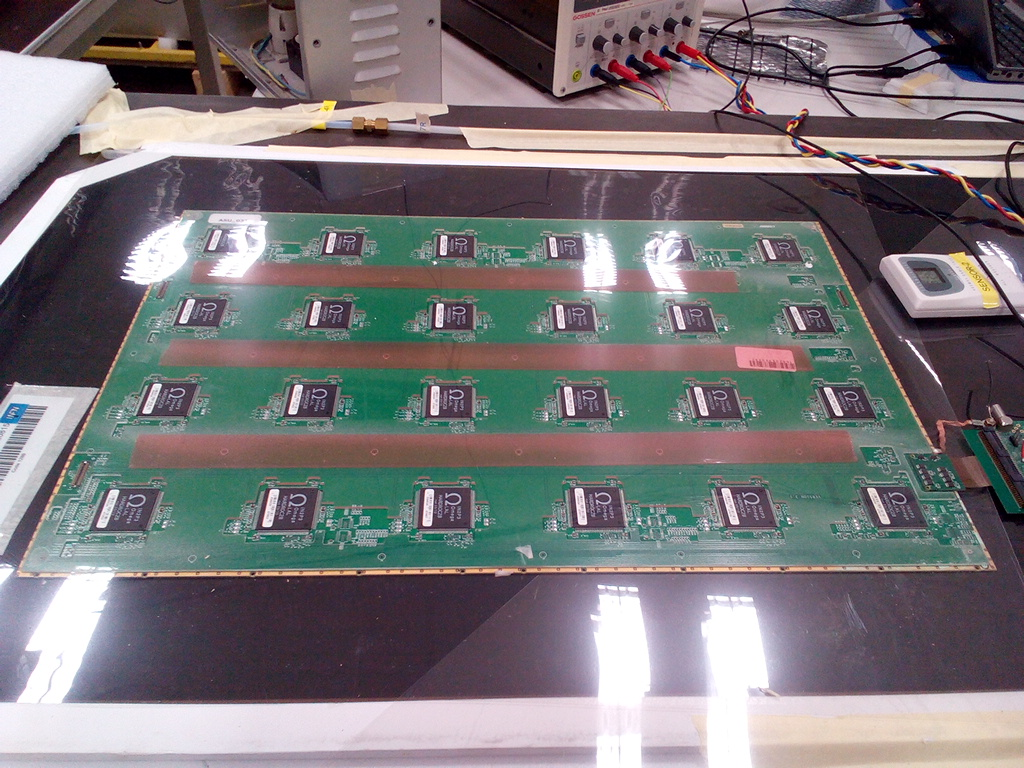
\includegraphics[width = \linewidth]{fig/chapt6/HARDROC_PCB.jpg}
			\caption{\label{fig:Setup-HARDROC2-904:A}}
		\end{subfigure}
		\begin{subfigure}{.5\linewidth}
		    \centering
			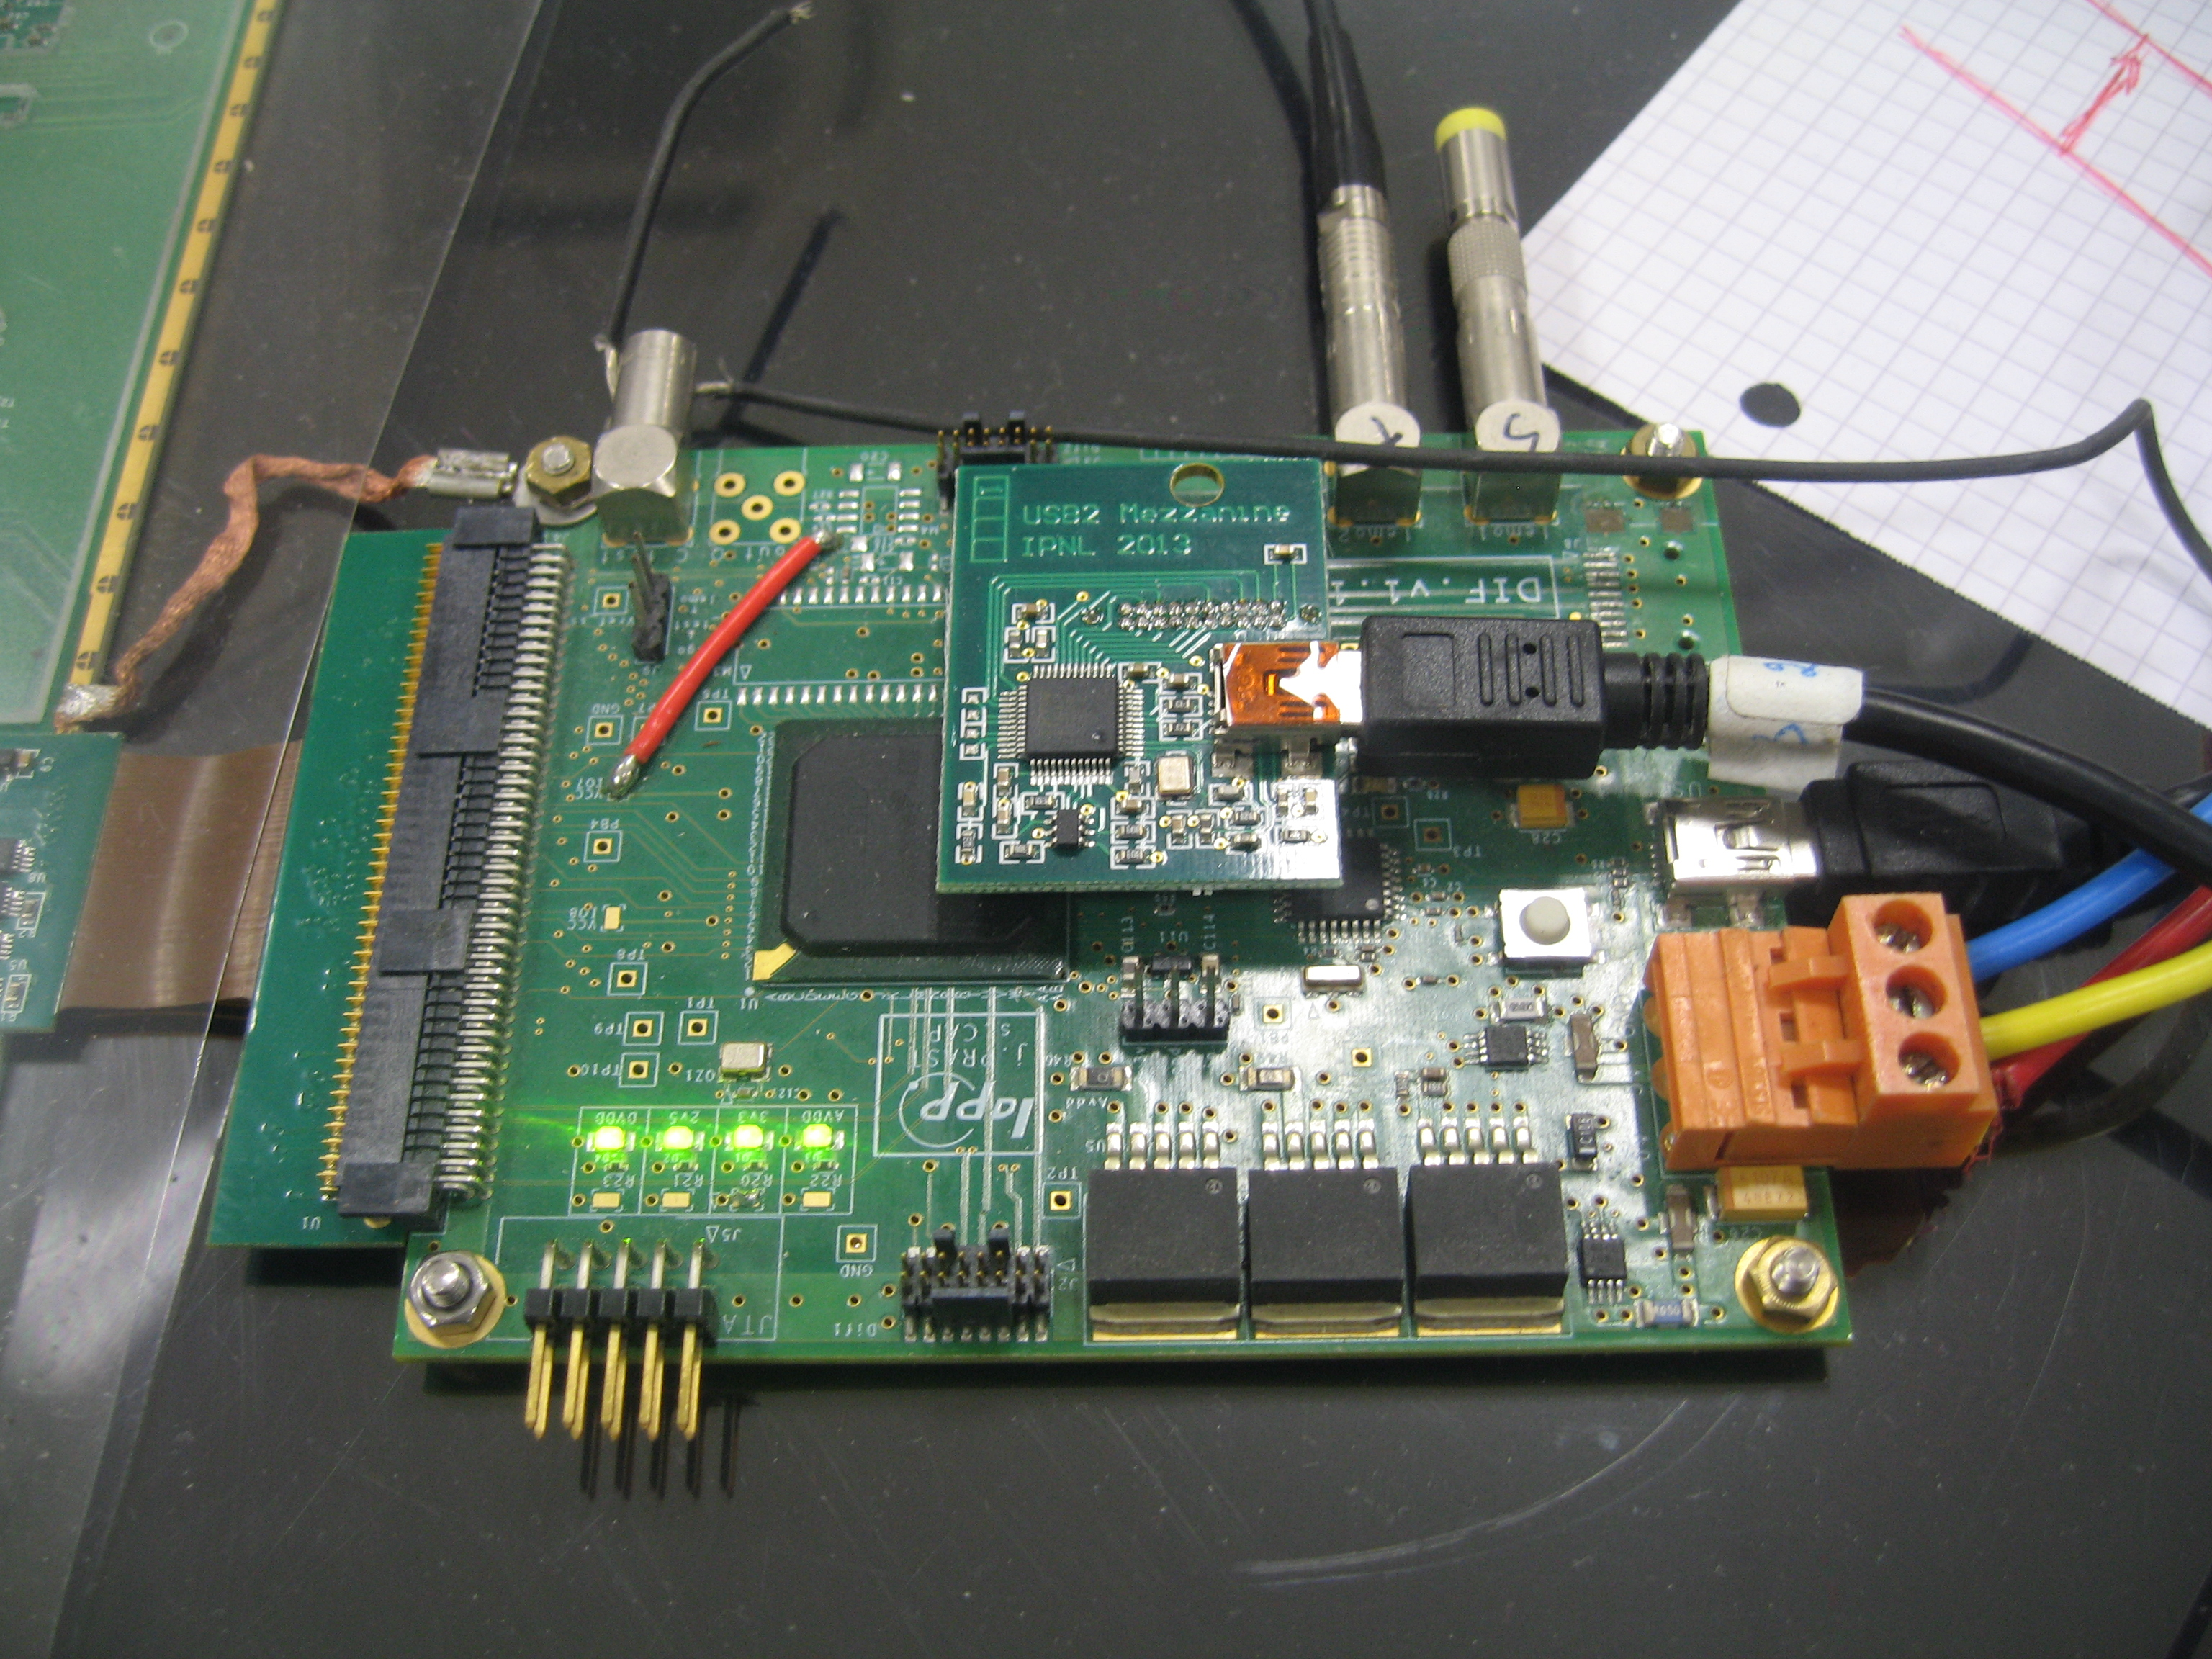
\includegraphics[width = \linewidth]{fig/chapt6/HARDROC_chip.JPG}
			\caption{\label{fig:Setup-HARDROC2-904:B}}
		\end{subfigure}
		\begin{subfigure}{\linewidth}
		    \centering
			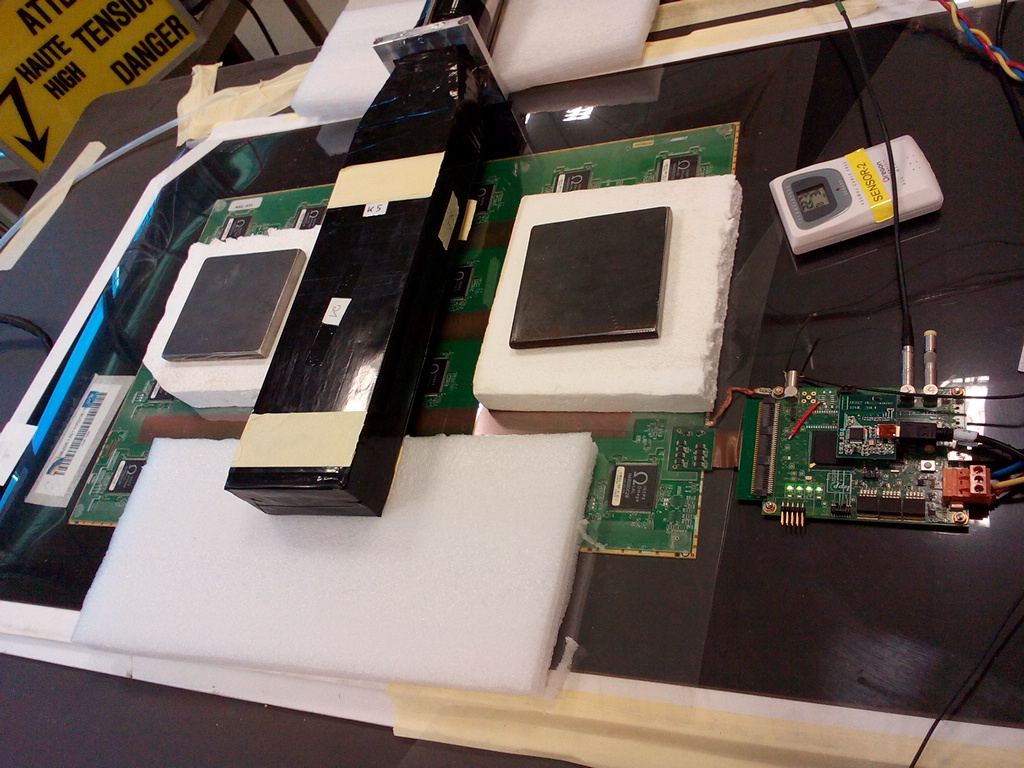
\includegraphics[width = 0.5\linewidth]{fig/chapt6/Setup_HARDROC_PAK.jpg}
			\caption{\label{fig:Setup-HARDROC2-904:C}}
		\end{subfigure}
		\caption{\label{fig:Setup-HARDROC2-904} Figure~ref{fig:Setup-HARDROC2-904:A}: Readout panel with the HARDROC2 ASIC placed on a CMS RPC gap. Figure~ref{fig:Setup-HARDROC2-904:B}: HARDROC2 control chip with its "Mezzanine" used to collect the data from the different HARDROC ASICs and communicate with the computer. Figure~ref{fig:Setup-HARDROC2-904:C}: Experimental setup used to test the HARDROC2 electronics.}
    \end{figure}
	
	\begin{figure}[H]
		\begin{subfigure}{.5\linewidth}
		    \centering
			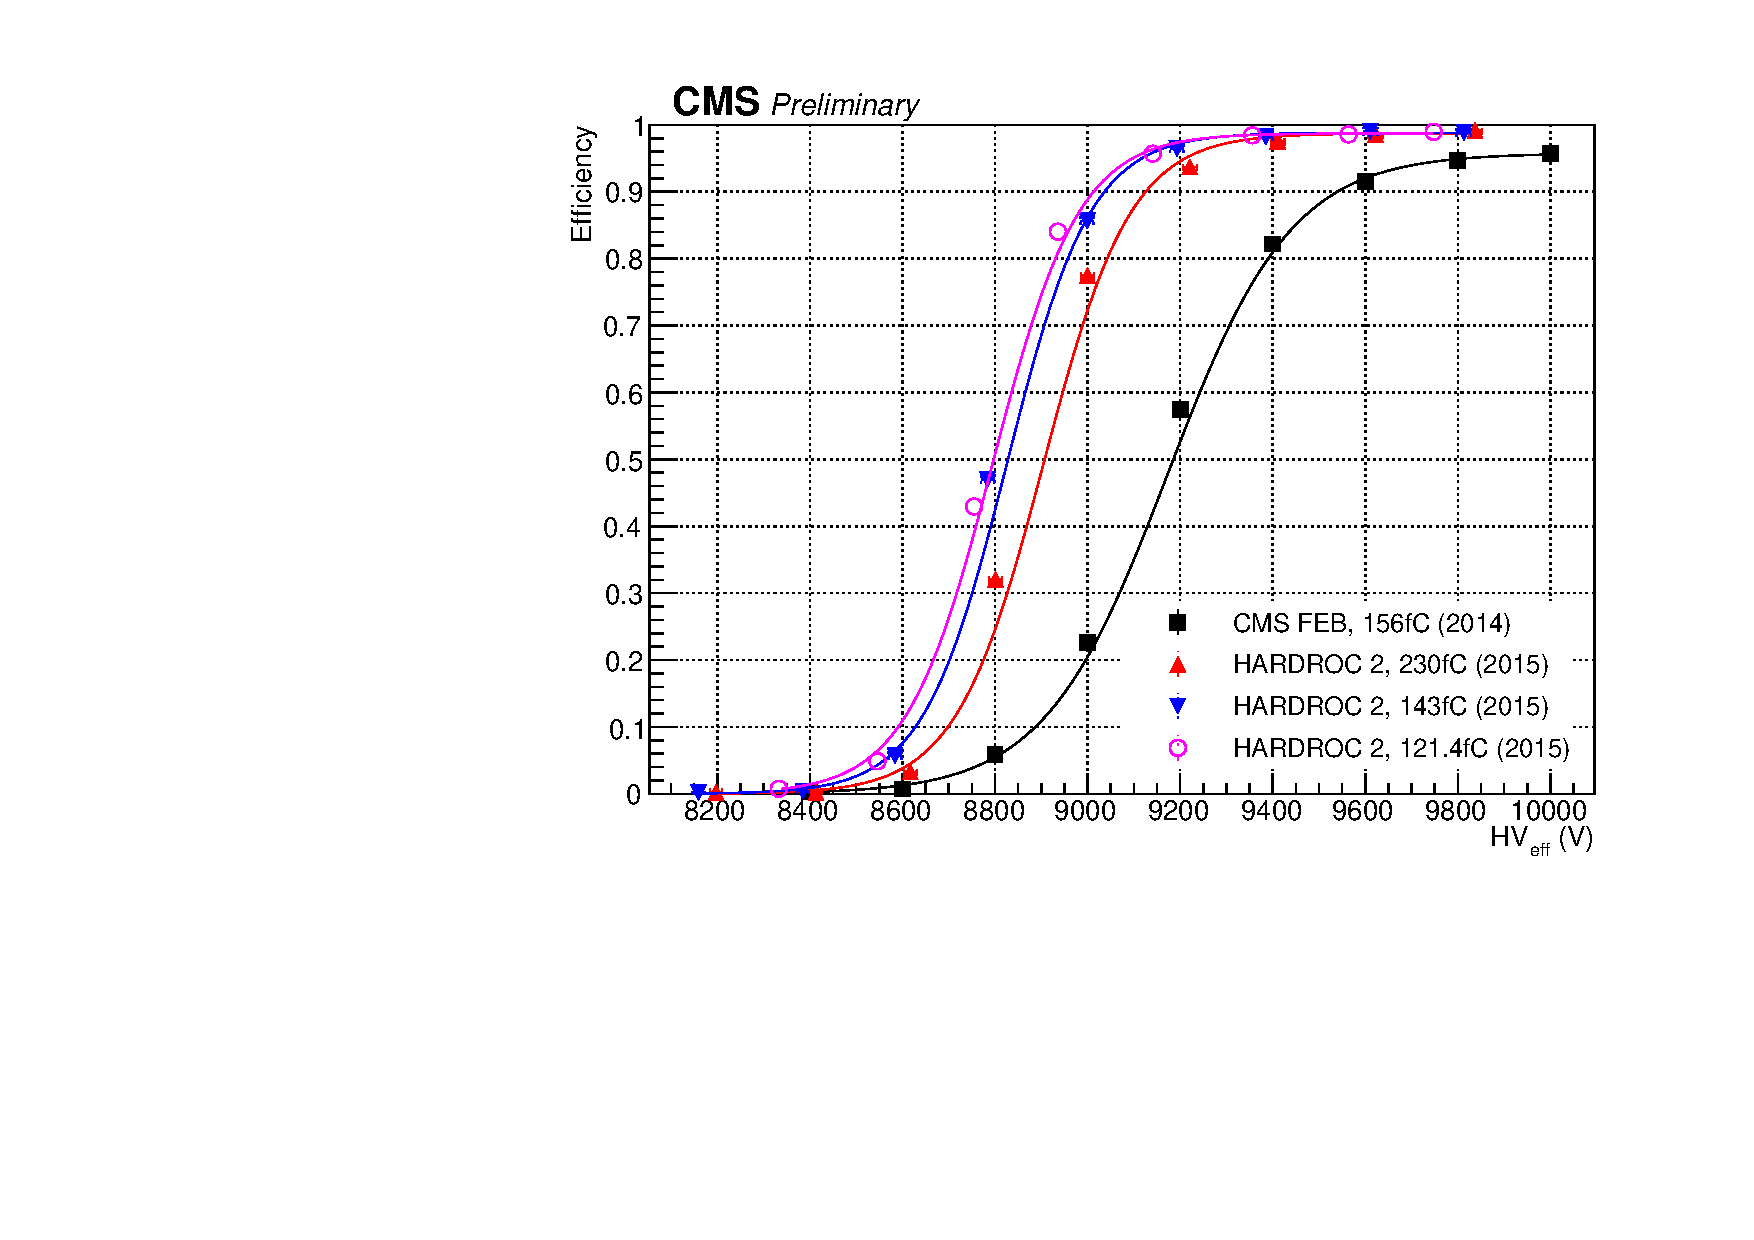
\includegraphics[width=\linewidth]{fig/chapt6/HARDROC2-Eff-Shift.pdf}
			\caption{\label{fig:HARDROC2:A}}
		\end{subfigure}
		\begin{subfigure}{.5\linewidth}
		    \centering
			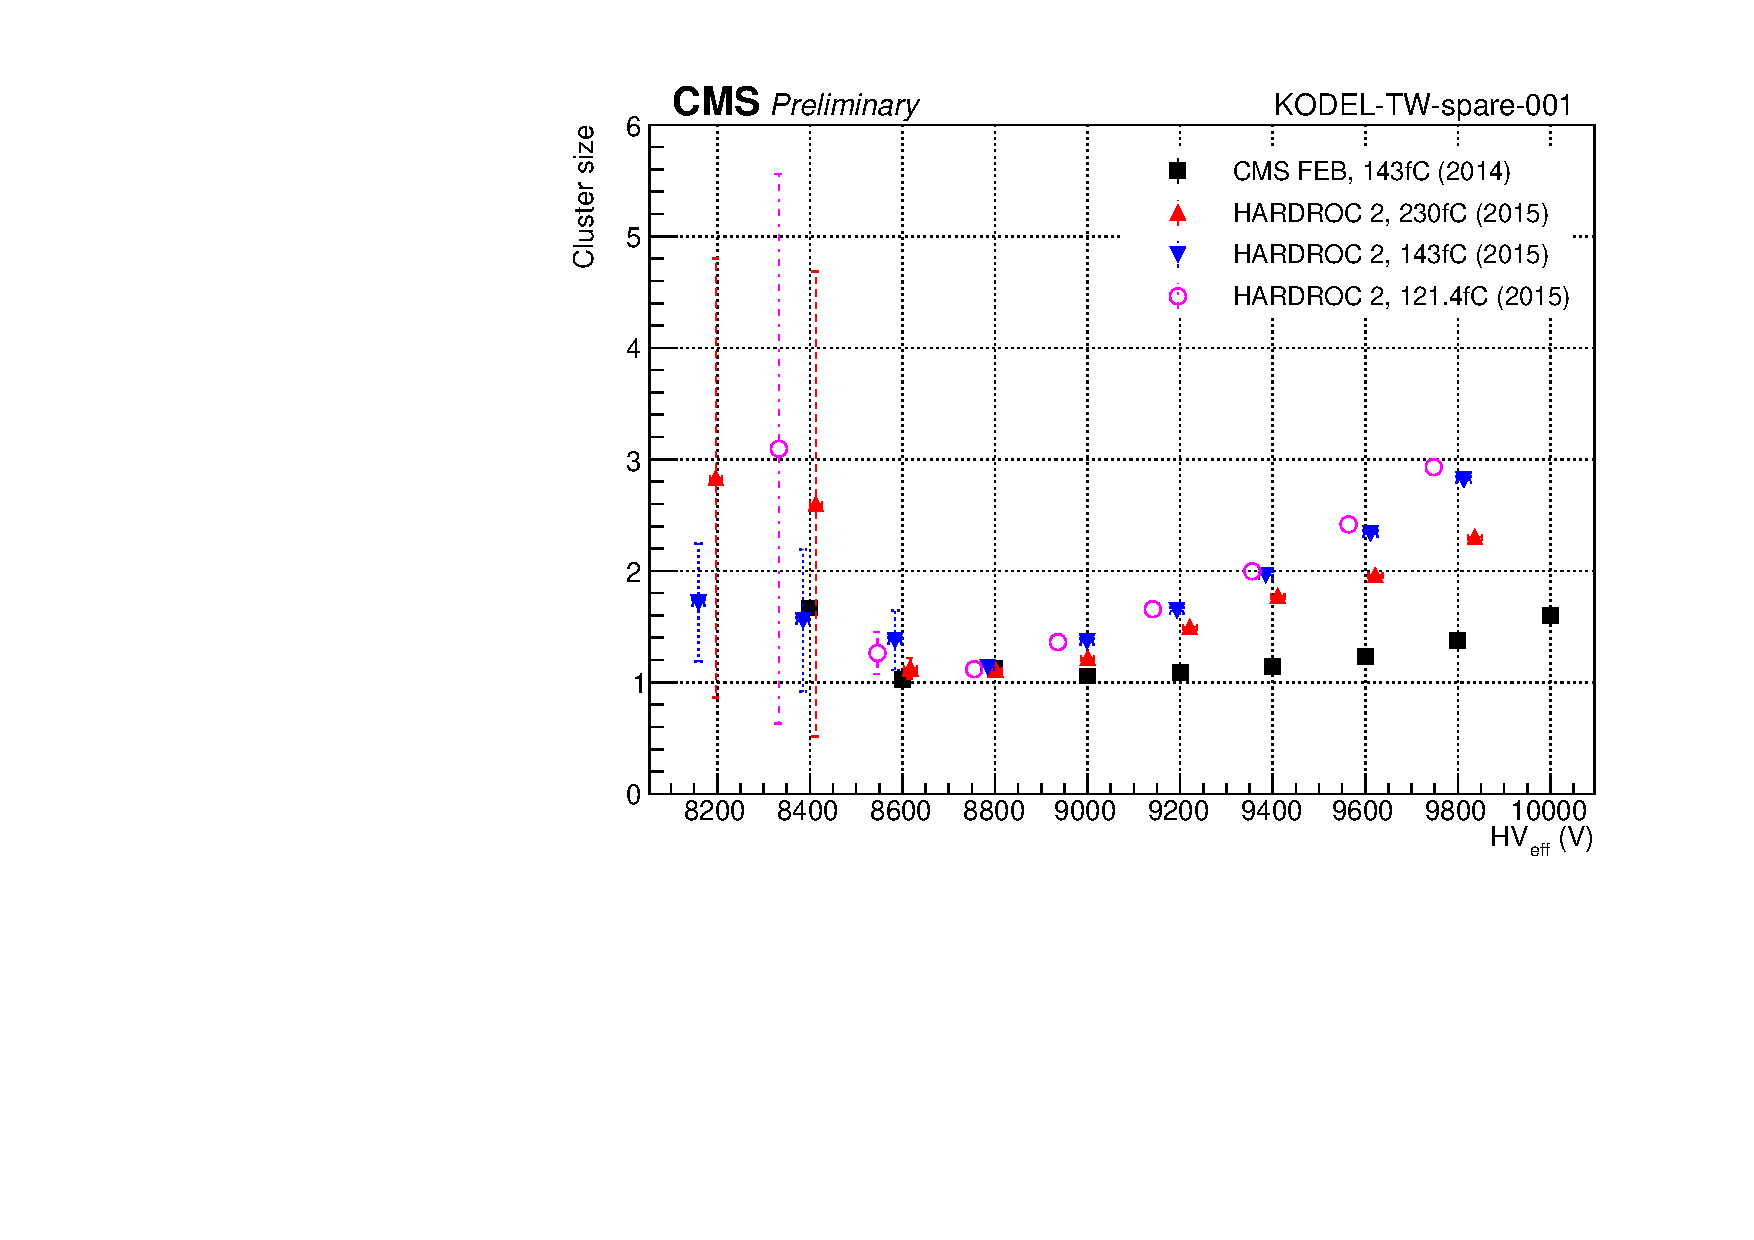
\includegraphics[width = \linewidth]{fig/chapt6/HARDROC2-ClS-Shift.pdf}
			\caption{\label{fig:HARDROC2:B}}
		\end{subfigure}
		\begin{subfigure}{\linewidth}
		    \centering
			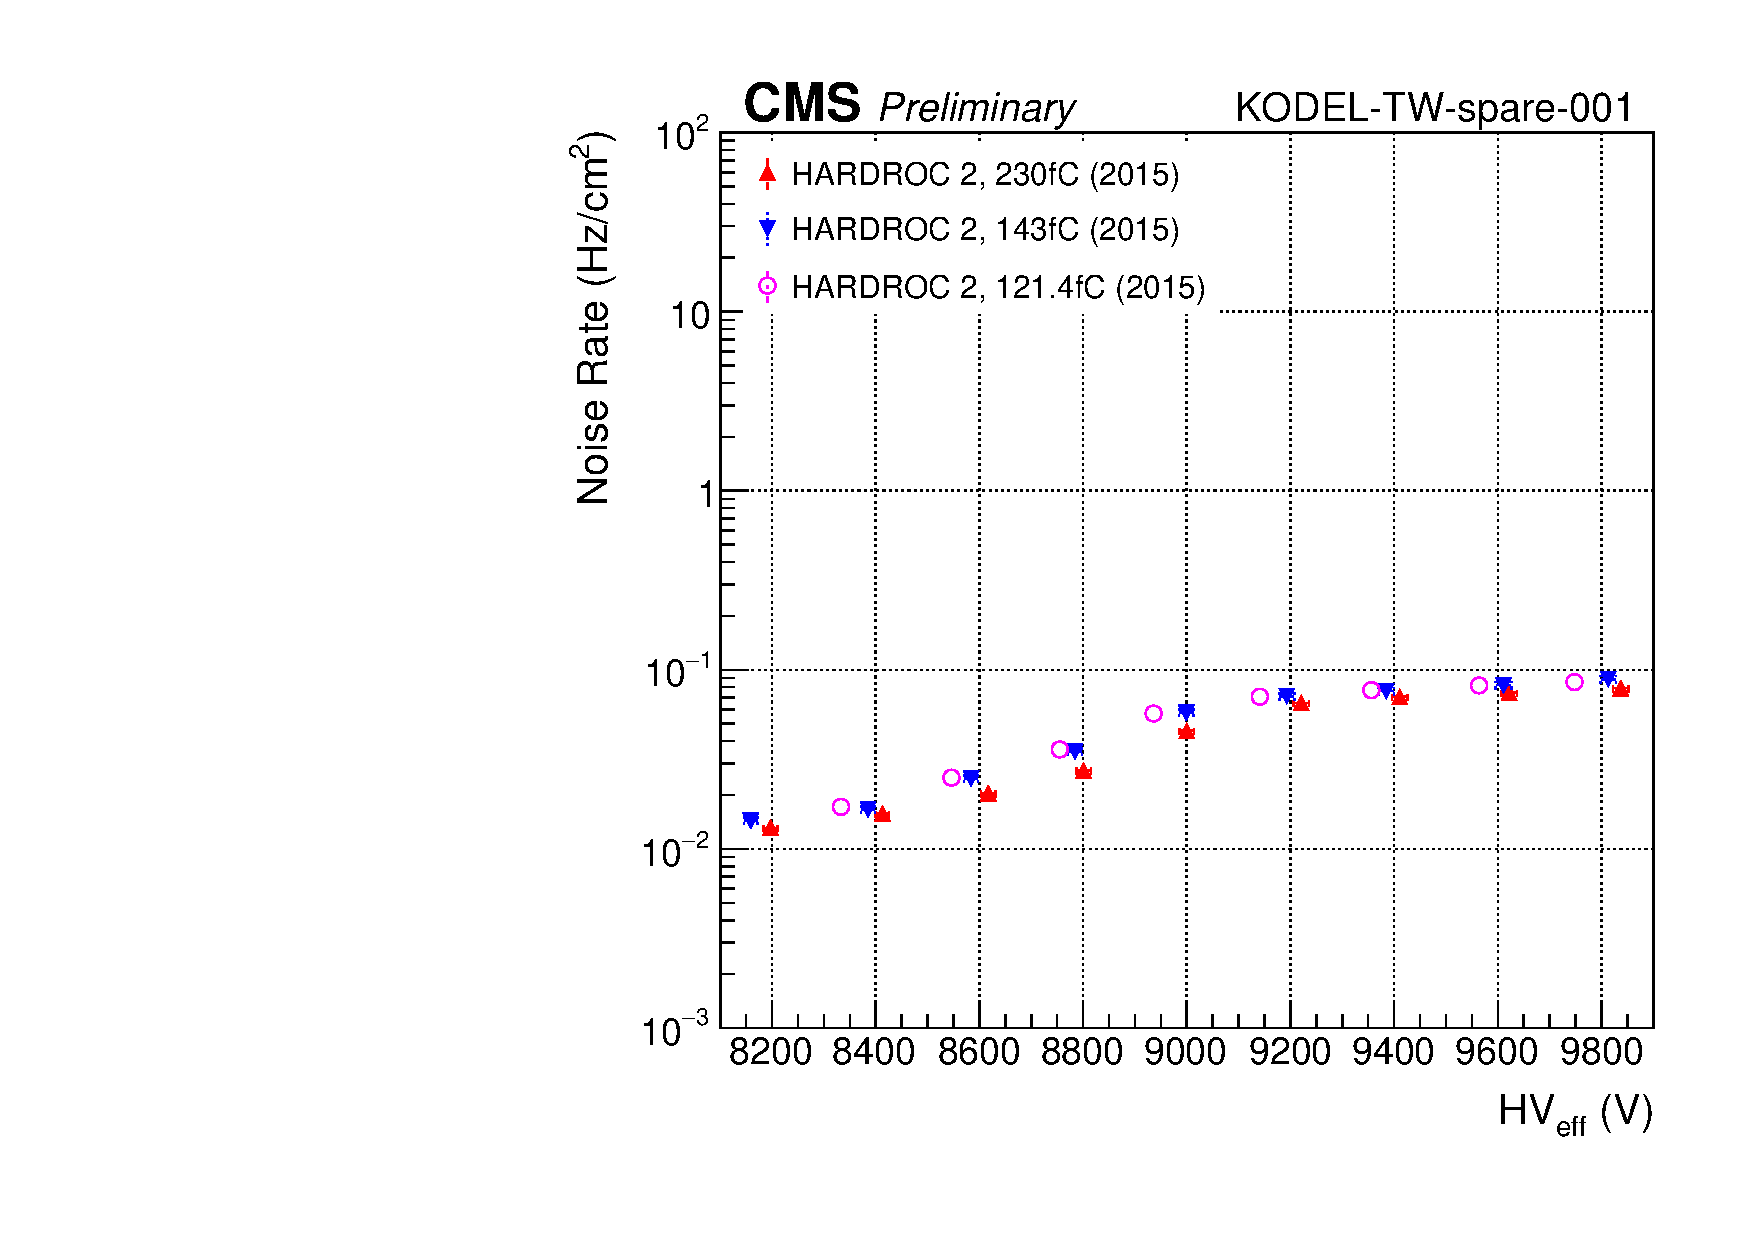
\includegraphics[width = .5\linewidth]{fig/chapt6/HARDROC2-Rate-Shift.pdf}
			\caption{\label{fig:HARDROC2:C}}
		\end{subfigure}
		\caption{\label{fig:HARDROC2} Efficiency (Figure~\ref{fig:HARDROC2:A}), cluster size (Figure~\ref{fig:HARDROC2:B}) and noise rate per unit area (Figure~\ref{fig:HARDROC2:C}) of the CMS RE4-3 detector tested with the standard CMS FEBs (black) and with the HARDROC 2 readout panel at different thresholds (red, blue and pink).}
	\end{figure}
	
	\begin{table}[H]
		\caption{\label{tab:HARDROC2} Results of the sigmoid fit (Formula~\ref{eq:Sigmoid}) performed on the data presented in Figure~\ref{fig:HARDROC2:A}. The working point and its corresponding efficiency are computed using Formula~\ref{eq:KneeWP}.}
		\footnotesize
		\begin{tabular}{|c|c|c|c|c|c|}
			\hline
			Data & $\epsilon_{max}$ & $\lambda$ ($\cdot$\Ord{-2} \si{V^{-1}}) & $HV_{50}$ (\si{V}) & $\epsilon_{WP}$ & $HV_{WP}$ (\si{V}) \\ 
			\hline
			CMS FEB, 156fC (2014) & \numerror{0.958}{0.000} & \numerror{0.75}{0.00} & \numerror{9174}{1} & \numerror{0.94}{0.00} & \numerror{9716}{2}\\ 
			\hline
			HARDROC 2, 230fC (2015) & \numerror{0.987}{0.002} & \numerror{1.06}{0.04} & \numerror{8905}{8} & \numerror{0.98}{0.01} & \numerror{9333}{17}\\ 
			\hline
			HARDROC 2, 143fC (2015) & \numerror{0.988}{0.001} & \numerror{1.10}{0.04} & \numerror{8826}{8} & \numerror{0.98}{0.01} & \numerror{9243}{17}\\ 
			\hline
			HARDROC 2, 121.4fC (2015) & \numerror{0.987}{0.001} & \numerror{1.07}{0.04} & \numerror{8795}{8} & \numerror{0.98}{0.01} & \numerror{9220}{17}\\ 
			\hline
		\end{tabular}
	\end{table}

\clearpage{\pagestyle{empty}\cleardoublepage}